\documentclass{beamer}

\usepackage{tikz}
\usepackage{amssymb}
\usepackage[utf8]{inputenc}

\usetikzlibrary {arrows.meta}
\usetikzlibrary{shapes.geometric}

\title{FUN with Complexity: Walking through Doors is Hard, even without Staircases}
\author{Manuel Frohn}
\institute{RWTH Aachen}
\date{2024}

\begin{document}



\frame{\titlepage}
\begin{frame}
  \frametitle{Content}
  \tableofcontents
\end{frame}
%1
\section{Theory}
\subsection{PSPACE-Complexity}
\begin{frame}
  \frametitle{PSPACE-Complexity}
  A given problem requires at most a polynomial amount of memory in relation to the
  input, to be solved $\Leftrightarrow$ The problem is in PSPACE
  \\~\\
  \begin{minipage}[t]{0.48\textwidth}
    \textbf{SAT}
    \[ x_1 \land x_2 \lor \lnot x_3 \]
  \end{minipage}
  \begin{minipage}[t]{0.48\textwidth}
    \textbf{Quantified SAT}
    \[ \forall x_1 \exists x_2 : x_1 \land x_2 \lor \lnot x_3 \]
  \end{minipage}
\end{frame}
%2
\subsection{1-PlayerMotionPlaning}
\begin{frame}
  \frametitle{1-PlayerMotionPlaning}
  Given: Enviroment, Agent, Goal \\
  Question: Is the goal achivable
  \\~\\
  \centerline{
    
\includegraphics[width=0.40\textwidth]{res/Maze.png}
    \hspace{2.5cm}
    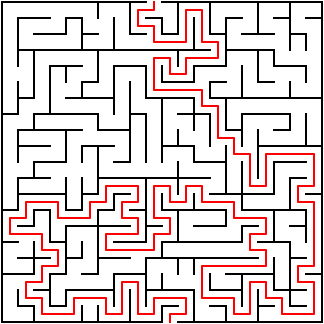
\includegraphics[width=0.40\textwidth]{res/MazeSolved.png}
  }
\end{frame}
%3
\subsection{Basic Door Device}
\begin{frame}
  \frametitle{Basic Door Device}
  \centerline{
    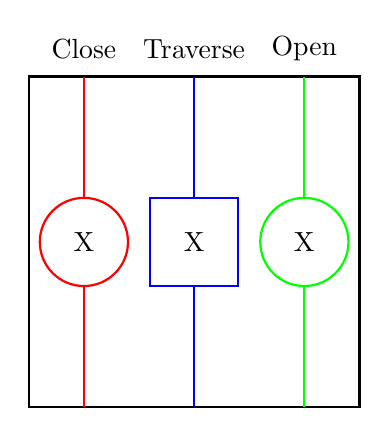
\begin{tikzpicture}[scale=0.7]
      \draw[thick] (0,0) rectangle (6,6);
      \node at (1,6.5) {Close};
      \node at (3,6.5) {Traverse};
      \node at (5,6.5) {Open};
      \def\shapesize{0.8}
      \draw[red, thick] (1,0) -- (1,3-\shapesize);
      \draw[red, thick] (1,3+\shapesize) -- (1,6);
      \draw[green, thick] (5,0) -- (5,3-\shapesize);
      \draw[green, thick] (5,3+\shapesize) -- (5,6);
      \draw[blue, thick] (3,0) -- (3,3-\shapesize);
      \draw[blue, thick] (3,3+\shapesize) -- (3,6);
      \draw[red, thick] (1,3) circle (\shapesize cm);
      \draw[green, thick] (5,3) circle (\shapesize cm);
      \draw[blue, thick] (3-\shapesize, 3-\shapesize) rectangle (3+\shapesize, 3+\shapesize);
      \node at (1,3) {X};
      \node at (3,3) {X};
      \node at (5,3) {X};

    \end{tikzpicture}
    \hspace{2.5cm}
    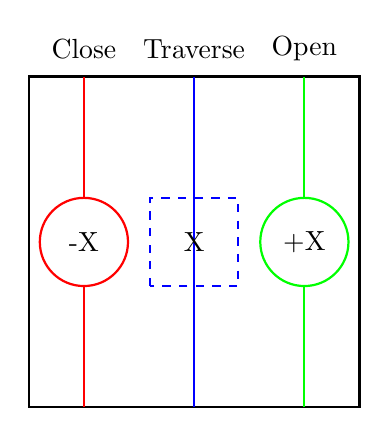
\begin{tikzpicture}[scale=0.7]
      \draw[thick] (0,0) rectangle (6,6);
      \node at (1,6.5) {Close};
      \node at (3,6.5) {Traverse};
      \node at (5,6.5) {Open};
      \def\shapesize{0.8}
      \draw[red, thick] (1,0) -- (1,3-\shapesize);
      \draw[red, thick] (1,3+\shapesize) -- (1,6);
      \draw[green, thick] (5,0) -- (5,3-\shapesize);
      \draw[green, thick] (5,3+\shapesize) -- (5,6);
      \draw[blue, thick] (3,0) -- (3,6);
      \draw[red, thick] (1,3) circle (\shapesize cm);
      \draw[green, thick] (5,3) circle (\shapesize cm);
      \draw[blue, thick, dashed] (3-\shapesize, 3-\shapesize) rectangle (3+\shapesize, 3+\shapesize);
      \node at (1,3) {-X};
      \node at (3,3) {X};
      \node at (5,3) {+X};

    \end{tikzpicture}
  }
\end{frame}
%4
\subsection{PSPACE-hardness of doors}
\begin{frame}
  \frametitle{PSPACE-hardness of doors}
  \begin{theorem}
    If a game features \textbf{door devices} which each are controled by an
    \textcolor{green}{open} and a \textcolor{red}{close} \textbf{preasure plate}
    and the agent has to navigate from entrance to exit, then the game is
    \textbf{PSPACE-hard}
  \end{theorem}
\end{frame}
%5
\begin{frame}
  \frametitle{PSPACE-hardness of doors - Proof}
  \begin{minipage}[t]{0.48\textwidth}
    \textbf{True Quantified SAT}
    \[ \forall x \exists y \exists z :  (\overline{x} \lor y \lor z) \land \]
    \[ (\overline{x} \lor \overline{y} \lor z) \land (\lor x \lor y \lor \overline{z}) \]
  \end{minipage}
  \begin{minipage}[t]{0.48\textwidth}
    \textbf{1-Player Motion Planning}
    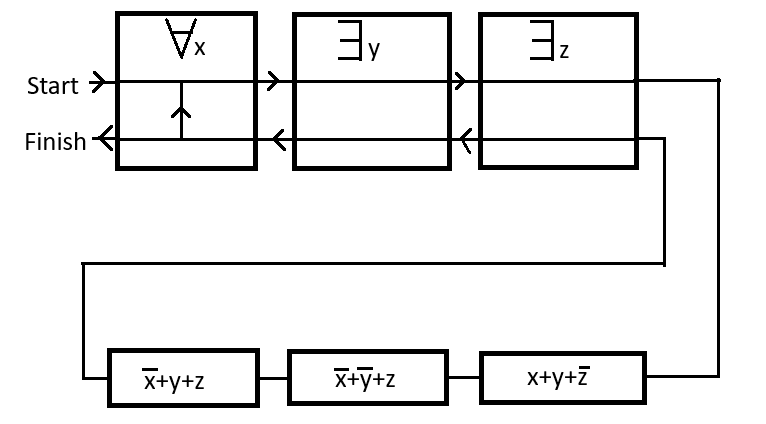
\includegraphics[width=1.20\textwidth]{res/prove/Conversion.png}
  \end{minipage}
\end{frame}

%6
\begin{frame}
  \frametitle{PSPACE-hardness of doors - Proof}
  \begin{minipage}[t]{0.45\textwidth}
    \textbf{Clause}
    \[ (\overline{x} \lor y \lor z) \]
  \end{minipage}
  \begin{minipage}[t]{0.45\textwidth}
    \textbf{Gadget}\\
    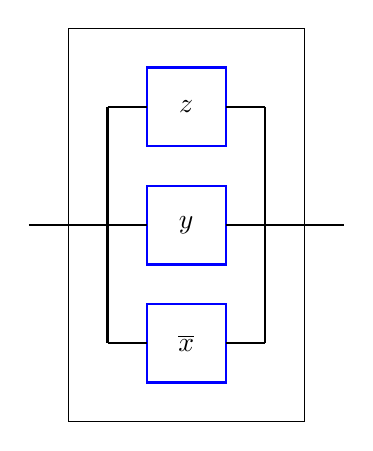
\begin{tikzpicture}
      \draw (0,0.5) rectangle (3,5.5);

      \node at (1.5,1.5) {$\overline{x}$};
      \draw[thick, blue] (1,1) rectangle (2,2);
      \node at (1.5,3) {$y$};
      \draw[thick, blue] (1,2.5) rectangle (2,3.5);
      \node at (1.5,4.5) {$z$};
      \draw[thick, blue] (1,4) rectangle (2,5);

      \draw[thick] (0.5, 1.5) -- (1,1.5);
      \draw[thick] (-0.5, 3) -- (1,3);
      \draw[thick] (0.5, 4.5) -- (1,4.5);
      \draw[thick] (0.5, 4.5) -- (0.5, 1.5);

      \draw[thick] (2, 1.5) -- (2.5,1.5);
      \draw[thick] (2, 3) -- (3.5,3);
      \draw[thick] (2, 4.5) -- (2.5,4.5);
      \draw[thick] (2.5,4.5) -- (2.5,1.5);
    \end{tikzpicture}
  \end{minipage}
\end{frame}

%7
\begin{frame}
  \frametitle{PSPACE-hardness of doors - Proof}
  \begin{minipage}[t]{0.45\textwidth}
    \textbf{Exists-Quantor}
    \[ \exists y \]\\
    Open preasure plate: \tikz\draw[green,fill=green] (0,0) circle (2mm);\\
    Close preasure plate: \tikz\draw[red,fill=red] (0,0) circle (2mm);\\
    Door: \tikz\draw[blue,fill=blue] (0.2,0.2) rectangle (0.6,0.6);
  \end{minipage}
  \begin{minipage}[t]{0.45\textwidth}
    \textbf{Gadget}
    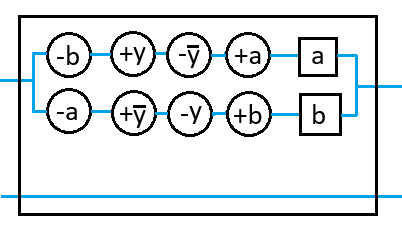
\includegraphics[width=1.3\textwidth]{res/prove/ExsistsGadget.png}
  \end{minipage}

\end{frame}

%8
\begin{frame}
  \frametitle{PSPACE-hardness of doors - Proof}
  \begin{minipage}[t]{0.45\textwidth}
    \textbf{All-Quantor}
    \[ \forall x \]\\
    Open preasure plate: \tikz\draw[green,fill=green] (0,0) circle (2mm);\\
    Close preasure plate: \tikz\draw[red,fill=red] (0,0) circle (2mm);\\
    Door: \tikz\draw[blue,fill=blue] (0.2,0.2) rectangle (0.6,0.6);\\
  \end{minipage}
  \begin{minipage}[t]{0.45\textwidth}
    \textbf{Gadget}\\
    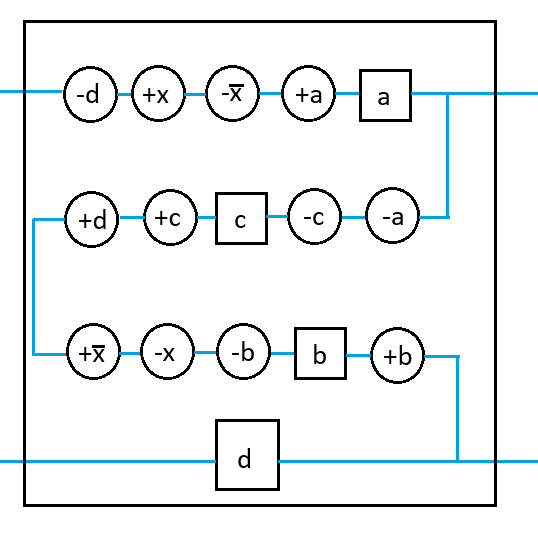
\includegraphics[width=1.3\textwidth]{res/prove/AllGadget.png}
  \end{minipage}

\end{frame}

\subsection{Door Device Variants}
%9
\begin{frame}
  \frametitle{Door Device - Variants}
  \begin{minipage}[b]{0.32\textwidth}
    \textbf{Basic}
    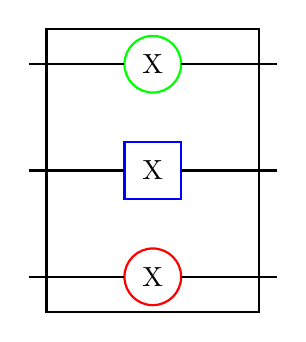
\begin{tikzpicture}[scale=0.45]
      \def\shapesize{0.8}

      \draw[thick] (0,0) rectangle (6,8);
      \node at (3,1) {X};
      \node at (3,4) {X};
      \node at (3,7) {X};
      \draw[red, thick] (3,1) circle (\shapesize cm);
      \draw[green, thick] (3,7) circle (\shapesize cm);
      \draw[blue, thick] (3-\shapesize, 4-\shapesize) rectangle (3+\shapesize, 4+\shapesize);

      \draw[thick] (-0.5,1) -- (3-\shapesize,1);
      \draw[thick] (3+\shapesize,1) -- (6.5,1);
      \draw[thick] (-0.5,4) -- (3-\shapesize,4);
      \draw[thick] (3+\shapesize,4) -- (6.5,4);
      \draw[thick] (-0.5,7) -- (3-\shapesize,7);
      \draw[thick] (3+\shapesize,7) -- (6.5,7);

    \end{tikzpicture}
  \end{minipage}
  \begin{minipage}[b]{0.32\textwidth}
    \textbf{Open-Optional}
    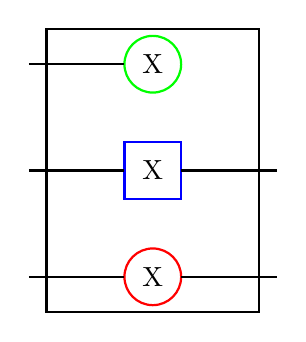
\begin{tikzpicture}[scale=0.45]
      \def\shapesize{0.8}

      \draw[thick] (0,0) rectangle (6,8);
      \node at (3,1) {X};
      \node at (3,4) {X};
      \node at (3,7) {X};
      \draw[red, thick] (3,1) circle (\shapesize cm);
      \draw[green, thick] (3,7) circle (\shapesize cm);
      \draw[blue, thick] (3-\shapesize, 4-\shapesize) rectangle (3+\shapesize, 4+\shapesize);

      \draw[thick] (-0.5,1) -- (3-\shapesize,1);
      \draw[thick] (3+\shapesize,1) -- (6.5,1);
      \draw[thick] (-0.5,4) -- (3-\shapesize,4);
      \draw[thick] (3+\shapesize,4) -- (6.5,4);
      \draw[thick] (-0.5,7) -- (3-\shapesize,7);

    \end{tikzpicture}
  \end{minipage}
  \begin{minipage}[b]{0.32\textwidth}
    \textbf{Directed}
    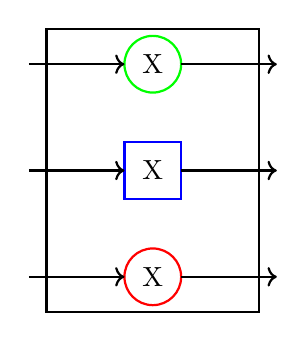
\begin{tikzpicture}[scale=0.45]
      \def\shapesize{0.8}

      \draw[thick] (0,0) rectangle (6,8);
      \node at (3,1) {X};
      \node at (3,4) {X};
      \node at (3,7) {X};
      \draw[red, thick] (3,1) circle (\shapesize cm);
      \draw[green, thick] (3,7) circle (\shapesize cm);
      \draw[blue, thick] (3-\shapesize, 4-\shapesize) rectangle (3+\shapesize, 4+\shapesize);

      \draw[thick, ->] (-0.5,1) -- (3-\shapesize,1);
      \draw[thick, ->] (3+\shapesize,1) -- (6.5,1);
      \draw[thick, ->] (-0.5,4) -- (3-\shapesize,4);
      \draw[thick, ->] (3+\shapesize,4) -- (6.5,4);
      \draw[thick, ->] (-0.5,7) -- (3-\shapesize,7);
      \draw[thick, ->] (3+\shapesize,7) -- (6.5,7);

    \end{tikzpicture}
  \end{minipage}
  Open preasure plate: \tikz\draw[green,fill=green] (0,0) circle (2mm);
  Close preasure plate: \tikz\draw[red,fill=red] (0,0) circle (2mm);
  Door: \tikz\draw[blue,fill=blue] (0.2,0.2) rectangle (0.6,0.6);
\end{frame}


\begin{frame}
  \frametitle{PSpace-Hardness - Open optinal door}
  \begin{minipage}[b]{0.49\textwidth}
    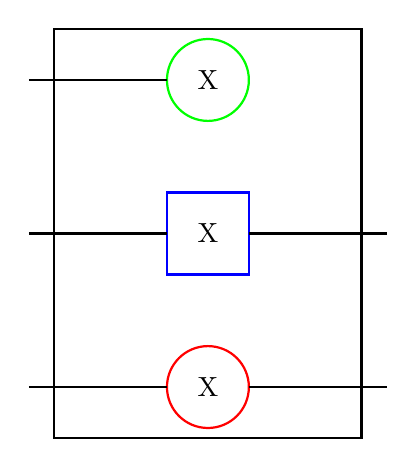
\begin{tikzpicture}[scale=0.65]
      \def\shapesize{0.8}

      \draw[thick] (0,0) rectangle (6,8);
      \node at (3,1) {X};
      \node at (3,4) {X};
      \node at (3,7) {X};
      \draw[red, thick] (3,1) circle (\shapesize cm);
      \draw[green, thick] (3,7) circle (\shapesize cm);
      \draw[blue, thick] (3-\shapesize, 4-\shapesize) rectangle (3+\shapesize, 4+\shapesize);

      \draw[thick] (-0.5,1) -- (3-\shapesize,1);
      \draw[thick] (3+\shapesize,1) -- (6.5,1);
      \draw[thick] (-0.5,4) -- (3-\shapesize,4);
      \draw[thick] (3+\shapesize,4) -- (6.5,4);
      \draw[thick] (-0.5,7) -- (3-\shapesize,7);

    \end{tikzpicture}
  \end{minipage}
  \begin{minipage}[b]{0.49\textwidth}
    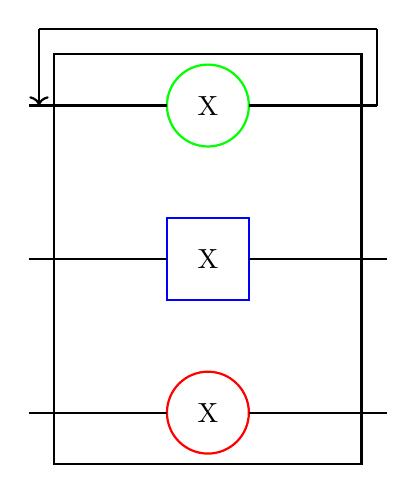
\begin{tikzpicture}[scale=0.65]
      \def\shapesize{0.8}

      \draw[thick] (0,0) rectangle (6,8);
      \node at (3,1) {X};
      \node at (3,4) {X};
      \node at (3,7) {X};
      \draw[red, thick] (3,1) circle (\shapesize cm);
      \draw[green, thick] (3,7) circle (\shapesize cm);
      \draw[blue, thick] (3-\shapesize, 4-\shapesize) rectangle (3+\shapesize, 4+\shapesize);

      \draw[thick] (-0.5,1) -- (3-\shapesize,1);
      \draw[thick] (3+\shapesize,1) -- (6.5,1);
      \draw[thick] (-0.5,4) -- (3-\shapesize,4);
      \draw[thick] (3+\shapesize,4) -- (6.5,4);
      \draw[thick] (-0.5,7) -- (3-\shapesize,7);
      \draw[thick] (3+\shapesize,7) -- (6.3,7);
      \draw[thick] (6.3,7) -- (6.3,8.5);
      \draw[thick] (-0.3,8.5) -- (6.3,8.5);
      \draw[thick, ->]  (-0.3,8.5) -- (-0.3,7);

    \end{tikzpicture}
  \end{minipage}
  Open preasure plate: \tikz\draw[green,fill=green] (0,0) circle (2mm);
  Close preasure plate: \tikz\draw[red,fill=red] (0,0) circle (2mm);
  Door: \tikz\draw[blue,fill=blue] (0.2,0.2) rectangle (0.6,0.6);
\end{frame}

\begin{frame}
  \frametitle{The Diode}
  \begin{minipage}[t]{0.49\textwidth}
    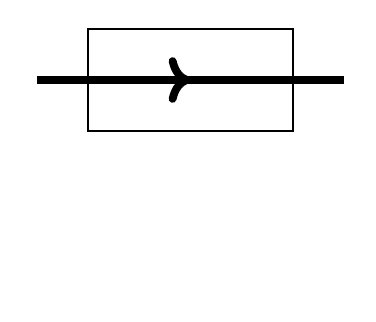
\begin{tikzpicture}[scale=0.65]
      \node at (0,0){};
      \draw[thick] (1,3) rectangle (5,5);
      \draw[thick, ->, line width=1mm] (0,4) -- (3,4);
      \draw[thick, line width=1mm] (2.5,4) -- (6,4);
    \end{tikzpicture}
  \end{minipage}
  \begin{minipage}[t]{0.49\textwidth}
    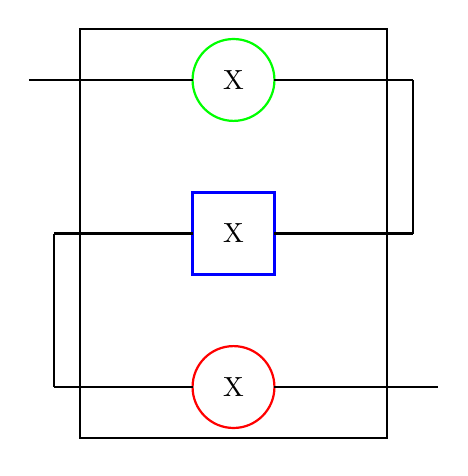
\begin{tikzpicture}[scale=0.65]
      \def\shapesize{0.8}
      \node at (0,0){};

      \draw[thick] (0,0) rectangle (6,8);
      \node at (3,1) {X};
      \node at (3,4) {X};
      \node at (3,7) {X};
      \draw[red, thick] (3,1) circle (\shapesize cm);
      \draw[green, thick] (3,7) circle (\shapesize cm);
      \draw[blue, thick] (3-\shapesize, 4-\shapesize) rectangle (3+\shapesize, 4+\shapesize);

      \draw[thick] (-0.5,1) -- (3-\shapesize,1);
      \draw[thick] (3+\shapesize,1) -- (7,1);
      \draw[thick] (-0.5,4) -- (3-\shapesize,4);
      \draw[thick] (3+\shapesize,4) -- (6.5,4);
      \draw[thick] (-1,7) -- (3-\shapesize,7);
      \draw[thick] (3+\shapesize,7) -- (6.5,7);

      \draw[thick] (6.5,7) -- (6.5,4);
      \draw[thick] (-0.5,4) -- (-0.5,1);
    \end{tikzpicture}
  \end{minipage}
  Open preasure plate: \tikz\draw[green,fill=green] (0,0) circle (2mm);
  Close preasure plate: \tikz\draw[red,fill=red] (0,0) circle (2mm);
  Door: \tikz\draw[blue,fill=blue] (0.2,0.2) rectangle (0.6,0.6);
\end{frame}

\begin{frame}
  \frametitle{PSpace-Hardness - Directed Door}
  \begin{minipage}[t]{0.49\textwidth}
    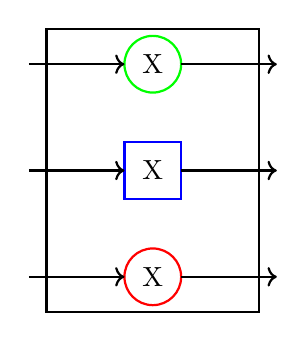
\begin{tikzpicture}[scale=0.45]
      \def\shapesize{0.8}

      \draw[thick] (0,0) rectangle (6,8);
      \node at (3,1) {X};
      \node at (3,4) {X};
      \node at (3,7) {X};
      \draw[red, thick] (3,1) circle (\shapesize cm);
      \draw[green, thick] (3,7) circle (\shapesize cm);
      \draw[blue, thick] (3-\shapesize, 4-\shapesize) rectangle (3+\shapesize, 4+\shapesize);

      \draw[thick, ->] (-0.5,1) -- (3-\shapesize,1);
      \draw[thick, ->] (3+\shapesize,1) -- (6.5,1);
      \draw[thick, ->] (-0.5,4) -- (3-\shapesize,4);
      \draw[thick, ->] (3+\shapesize,4) -- (6.5,4);
      \draw[thick, ->] (-0.5,7) -- (3-\shapesize,7);
      \draw[thick, ->] (3+\shapesize,7) -- (6.5,7);

    \end{tikzpicture}
  \end{minipage}
  \begin{minipage}[t]{0.49\textwidth}
    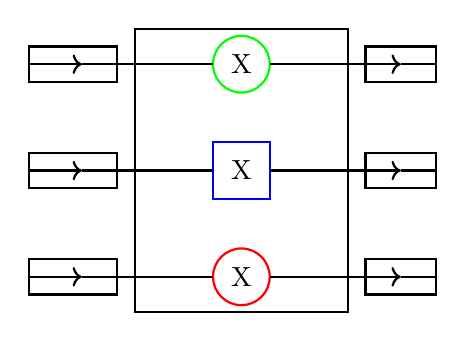
\begin{tikzpicture}[scale=0.45]
      \def\shapesize{0.8}

      \draw[thick] (0,0) rectangle (6,8);
      \node at (3,1) {X};
      \node at (3,4) {X};
      \node at (3,7) {X};
      \draw[red, thick] (3,1) circle (\shapesize cm);
      \draw[green, thick] (3,7) circle (\shapesize cm);
      \draw[blue, thick] (3-\shapesize, 4-\shapesize) rectangle (3+\shapesize, 4+\shapesize);

      \draw[thick] (-3,0.5) rectangle (-0.5,1.5);
      \draw[thick] (-1.5,1) -- (-0.5,1);
      \draw[thick, ->] (-3,1) -- (-1.5,1);
      \draw[thick] (-0.5,1) -- (3-\shapesize,1);

      \draw[thick] (6.5,0.5) rectangle (8.5, 1.5);
      \draw[thick, ->] (6.5,1) -- (7.5,1);
      \draw[thick] (7.5,1) -- (8.5,1);
      \draw[thick] (3+\shapesize,1) -- (6.5,1);

      \draw[thick] (-3,3.5) rectangle (-0.5,4.5);
      \draw[thick] (-1.5,4) -- (-0.5,4);
      \draw[thick, ->] (-3,4) -- (-1.5,4);
      \draw[thick] (-0.5,4) -- (3-\shapesize,4);

      \draw[thick] (6.5,3.5) rectangle (8.5, 4.5);
      \draw[thick, ->] (6.5,4) -- (7.5,4);
      \draw[thick] (7.5,4) -- (8.5,4);
      \draw[thick] (3+\shapesize,4) -- (6.5,4);

      \draw[thick] (-3,6.5) rectangle (-0.5,7.5);
      \draw[thick] (-1.5,7) -- (-0.5,7);
      \draw[thick, ->] (-3,7) -- (-1.5,7);
      \draw[thick] (-0.5,7) -- (3-\shapesize,7);

      \draw[thick] (6.5,6.5) rectangle (8.5, 7.5);
      \draw[thick, ->] (6.5,7) -- (7.5,7);
      \draw[thick] (7.5,7) -- (8.5,7);
      \draw[thick] (3+\shapesize,7) -- (6.5,7);

    \end{tikzpicture}
  \end{minipage}
  Open preasure plate: \tikz\draw[green,fill=green] (0,0) circle (2mm);
  Close preasure plate: \tikz\draw[red,fill=red] (0,0) circle (2mm);
  Door: \tikz\draw[blue,fill=blue] (0.2,0.2) rectangle (0.6,0.6);
\end{frame}

\begin{frame}
  \frametitle{Self closing doors}
  \begin{center}
    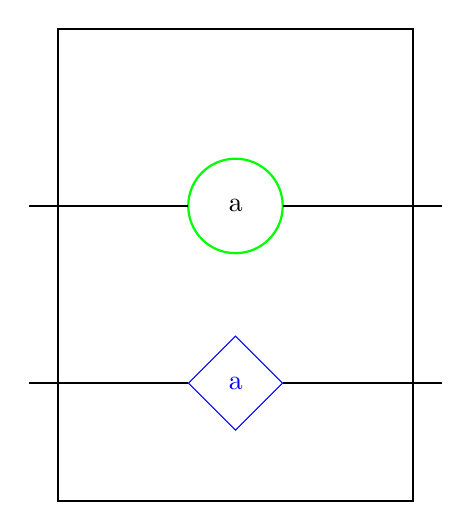
\begin{tikzpicture}[scale=0.75]
      \def\shapesize{0.8}


      \draw[thick] (0,0) rectangle (6,8);
      \node at (3,5) {a};
      \draw[green, thick] (3,5) circle (\shapesize cm);
      \node [draw, diamond, blue, 	minimum width = 1.2cm, minimum height = 1.2cm] at(3, 2){a};

      \draw[thick] (-0.5,5) -- (3-\shapesize,5);
      \draw[thick] (3+\shapesize,5) -- (6.5,5);
      \draw[thick] (-0.5,2) -- (3-\shapesize,2);
      \draw[thick] (3+\shapesize,2) -- (6.5,2);

    \end{tikzpicture}
  \end{center}
\end{frame}


\begin{frame}
  \frametitle{Self closing doors - Variants}

  \begin{minipage}[b]{0.32\textwidth}
    \textbf{Directed}
    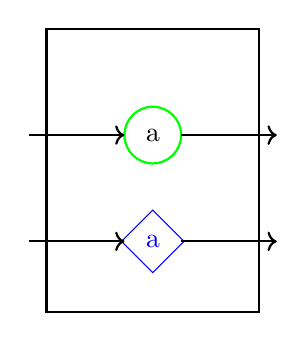
\begin{tikzpicture}[scale=0.45]
      \def\shapesize{0.8}


      \draw[thick] (0,0) rectangle (6,8);
      \node at (3,5) {a};
      \draw[green, thick] (3,5) circle (\shapesize cm);
      \node [draw, diamond, blue, 	minimum width = 0.8cm, minimum height = 0.8cm] at(3, 2){a};

      \draw[thick, ->] (-0.5,5) -- (3-\shapesize,5);
      \draw[thick, ->] (3+\shapesize,5) -- (6.5,5);
      \draw[thick, ->] (-0.5,2) -- (3-\shapesize,2);
      \draw[thick, ->] (3+\shapesize,2) -- (6.5,2);

    \end{tikzpicture}
  \end{minipage}
  \begin{minipage}[b]{0.32\textwidth}
    \textbf{Open-Optional}s
    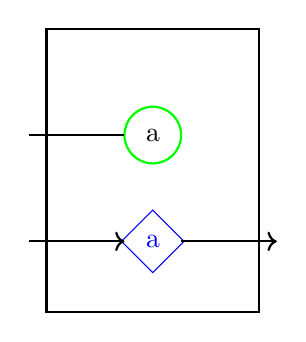
\begin{tikzpicture}[scale=0.45]
      \def\shapesize{0.8}


      \draw[thick] (0,0) rectangle (6,8);
      \node at (3,5) {a};
      \draw[green, thick] (3,5) circle (\shapesize cm);
      \node [draw, diamond, blue, 	minimum width = 0.8cm, minimum height = 0.8cm] at(3, 2){a};

      \draw[thick] (-0.5,5) -- (3-\shapesize,5);
      \draw[thick, ->] (-0.5,2) -- (3-\shapesize,2);
      \draw[thick, ->] (3+\shapesize,2) -- (6.5,2);

    \end{tikzpicture}
  \end{minipage}
  \begin{minipage}[b]{0.32\textwidth}
    \textbf{Symetric}
    \only<1>{
      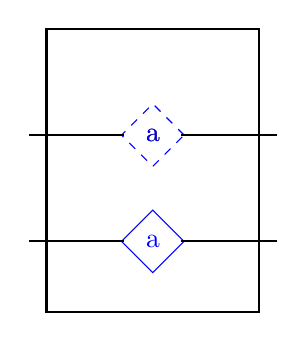
\begin{tikzpicture}[scale=0.45]

        \def\shapesize{0.8}


        \draw[thick] (0,0) rectangle (6,8);
        \node at (3,5) {a};
        \node [draw, diamond, blue, 	minimum width = 0.8cm, minimum height = 0.8cm, dashed] at(3, 5){a};
        \node [draw, diamond, blue, 	minimum width = 0.8cm, minimum height = 0.8cm] at(3, 2){a};

        \draw[thick] (-0.5,5) -- (3-\shapesize,5);
        \draw[thick] (3+\shapesize,5) -- (6.5,5);
        \draw[thick] (-0.5,2) -- (3-\shapesize,2);
        \draw[thick] (3+\shapesize,2) -- (6.5,2);

      \end{tikzpicture}
    }
    \only<2>{
      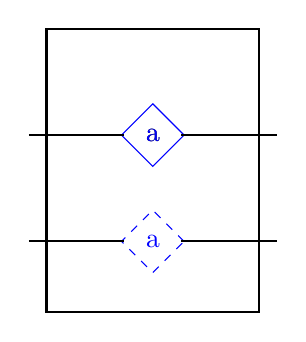
\begin{tikzpicture}[scale=0.45]

        \def\shapesize{0.8}


        \draw[thick] (0,0) rectangle (6,8);
        \node at (3,5) {a};
        \node [draw, diamond, blue, 	minimum width = 0.8cm, minimum height = 0.8cm] at(3, 5){a};
        \node [draw, diamond, blue, 	minimum width = 0.8cm, minimum height = 0.8cm, dashed] at(3, 2){a};

        \draw[thick] (-0.5,5) -- (3-\shapesize,5);
        \draw[thick] (3+\shapesize,5) -- (6.5,5);
        \draw[thick] (-0.5,2) -- (3-\shapesize,2);
        \draw[thick] (3+\shapesize,2) -- (6.5,2);

      \end{tikzpicture}
    }
  \end{minipage}
  Open preasure plate: \tikz\draw[green,fill=green] (0,0) circle (2mm);
  Self closing door: \tikz\node[blue,fill=blue, diamond] at (0,0){};
\end{frame}

\section{Application}
\subsection{Socobond is PSPACE-Hard}
\begin{frame}
  \frametitle{Application - Sokobond}

  \only<1>{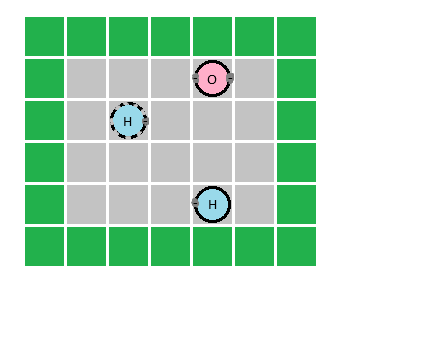
\includegraphics[width=1.2\textwidth]{res/SokobondIntro.png}}
  \only<2>{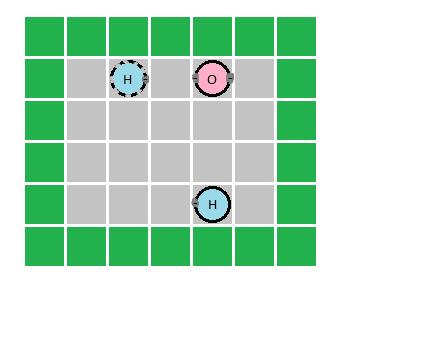
\includegraphics[width=1.2\textwidth]{res/SokobondIntro1.png}}
  \only<3>{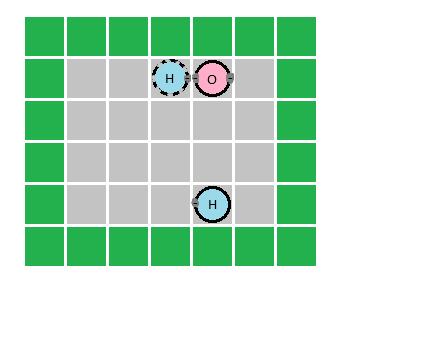
\includegraphics[width=1.2\textwidth]{res/SokobondIntro2.png}}
  \only<4>{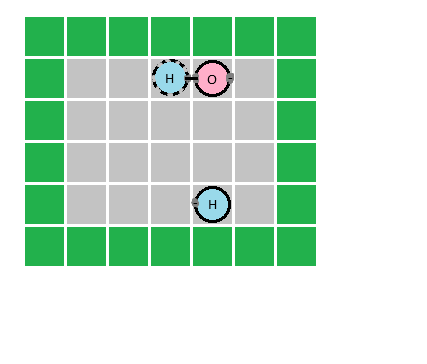
\includegraphics[width=1.2\textwidth]{res/SokobondIntro3.png}}
  \only<5>{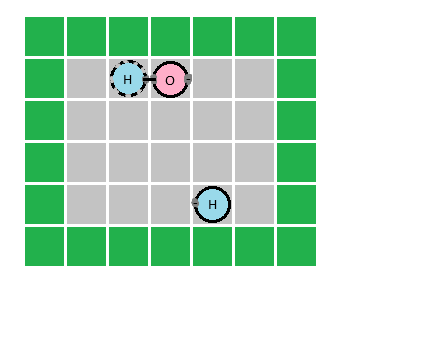
\includegraphics[width=1.2\textwidth]{res/SokobondIntro4.png}}
  \only<6>{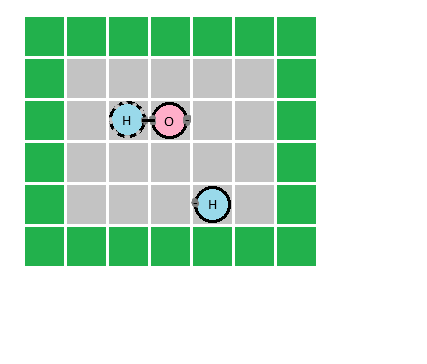
\includegraphics[width=1.2\textwidth]{res/SokobondIntro5.png}}
  \only<7>{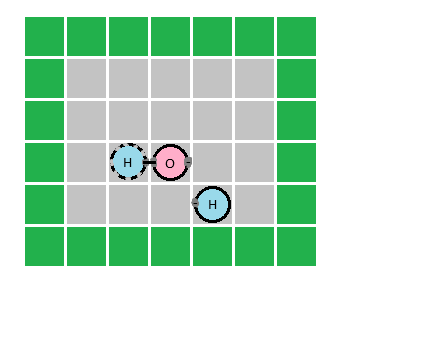
\includegraphics[width=1.2\textwidth]{res/SokobondIntro6.png}}
  \only<8>{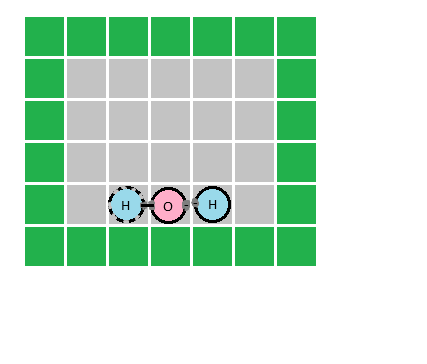
\includegraphics[width=1.2\textwidth]{res/SokobondIntro7.png}}
  \only<9>{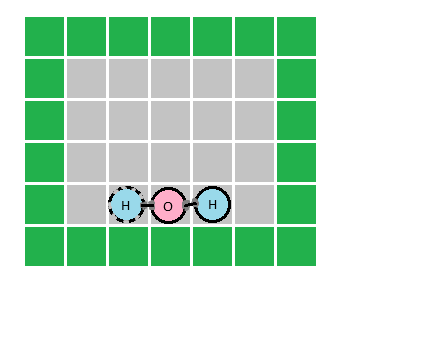
\includegraphics[width=1.2\textwidth]{res/SokobondIntro8.png}}
\end{frame}

\begin{frame}
  \frametitle{Sokobond is PSpace-Hard}
  \begin{minipage}[t]{0.49\textwidth}
    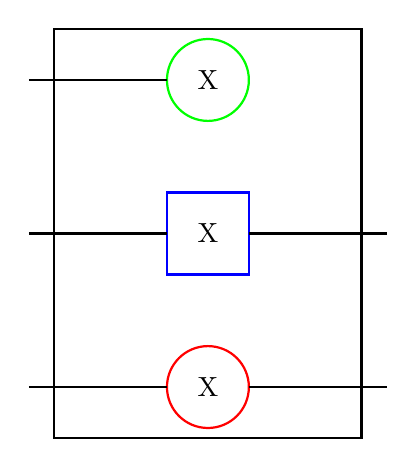
\begin{tikzpicture}[scale=0.65]
      \def\shapesize{0.8}

      \draw[thick] (0,0) rectangle (6,8);
      \node at (3,1) {X};
      \node at (3,4) {X};
      \node at (3,7) {X};
      \draw[red, thick] (3,1) circle (\shapesize cm);
      \draw[green, thick] (3,7) circle (\shapesize cm);
      \draw[blue, thick] (3-\shapesize, 4-\shapesize) rectangle (3+\shapesize, 4+\shapesize);

      \draw[thick] (-0.5,1) -- (3-\shapesize,1);
      \draw[thick] (3+\shapesize,1) -- (6.5,1);
      \draw[thick] (-0.5,4) -- (3-\shapesize,4);
      \draw[thick] (3+\shapesize,4) -- (6.5,4);
      \draw[thick] (-0.5,7) -- (3-\shapesize,7);

    \end{tikzpicture}
  \end{minipage}
  \begin{minipage}[t]{0.49\textwidth}
    \only<1>{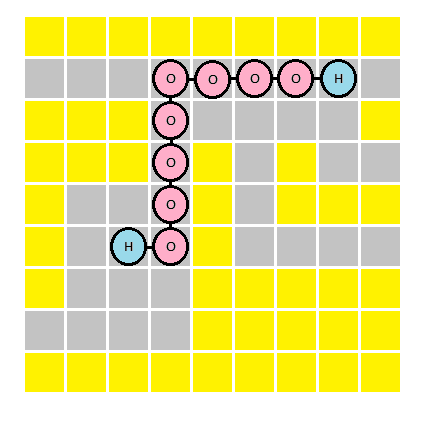
\includegraphics[width=1\textwidth]{res/SokobondProof.png}}
    \only<2>{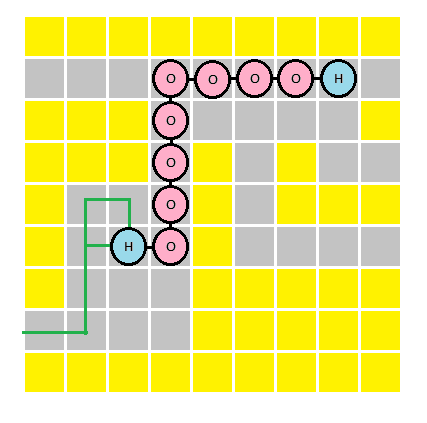
\includegraphics[width=1\textwidth]{res/SokobondProof1.png}}
    \only<3>{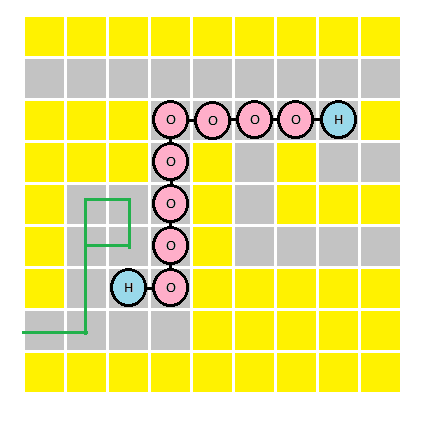
\includegraphics[width=1\textwidth]{res/SokobondProof2.png}}
    \only<4>{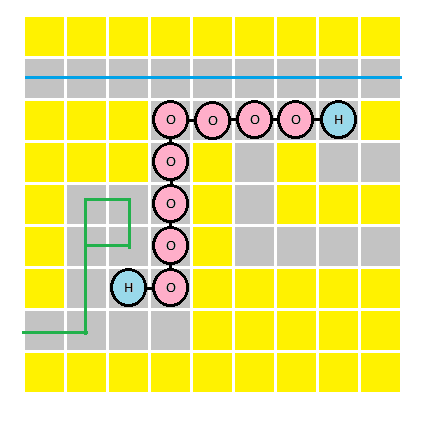
\includegraphics[width=1\textwidth]{res/SokobondProof3.png}}
    \only<5>{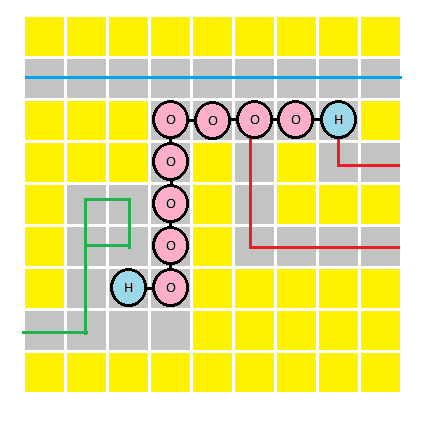
\includegraphics[width=1\textwidth]{res/SokobondProof4.png}}
    \only<6>{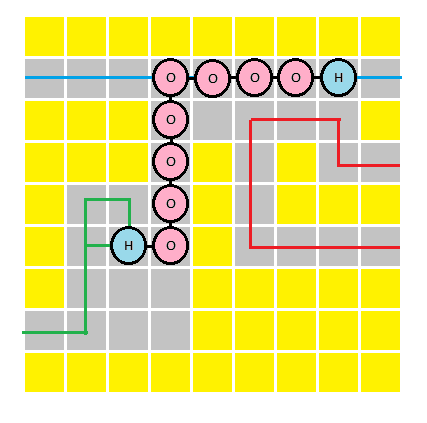
\includegraphics[width=1\textwidth]{res/SokobondProof5.png}}
  \end{minipage}
\end{frame}

\begin{frame}
  \frametitle{Reminder - Symetric self closing door}
  \begin{center}


    \only<1>{
      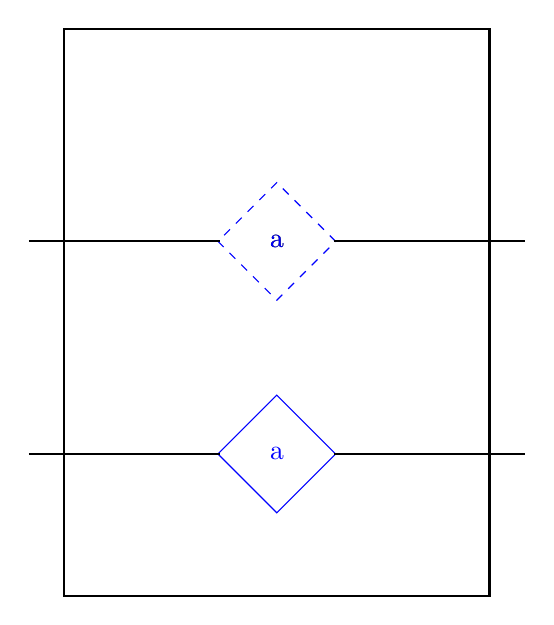
\begin{tikzpicture}[scale=.9]

        \def\shapesize{0.8}


        \draw[thick] (0,0) rectangle (6,8);
        \node at (3,5) {a};
        \node [draw, diamond, blue, 	minimum width = 1.5cm, minimum height = 1.5cm, dashed] at(3, 5){a};
        \node [draw, diamond, blue, 	minimum width = 1.5cm, minimum height = 1.5cm] at(3, 2){a};

        \draw[thick] (-0.5,5) -- (3-\shapesize,5);
        \draw[thick] (3+\shapesize,5) -- (6.5,5);
        \draw[thick] (-0.5,2) -- (3-\shapesize,2);
        \draw[thick] (3+\shapesize,2) -- (6.5,2);

      \end{tikzpicture}
    }
    \only<2>{
      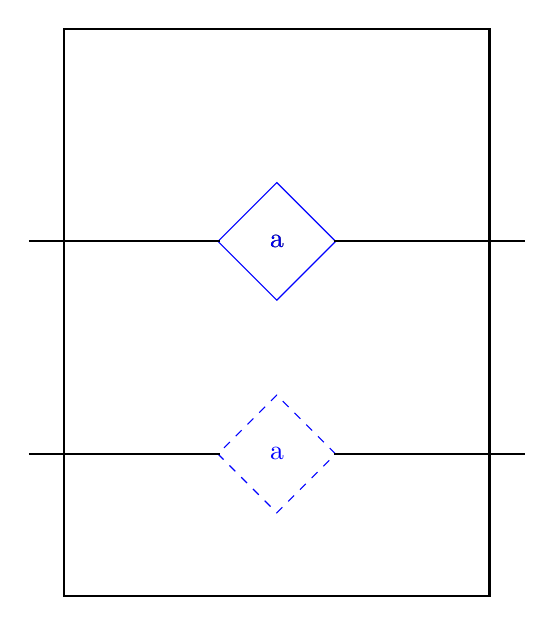
\begin{tikzpicture}[scale=.9]

        \def\shapesize{0.8}


        \draw[thick] (0,0) rectangle (6,8);
        \node at (3,5) {a};
        \node [draw, diamond, blue, 	minimum width = 1.5cm, minimum height = 1.5cm] at(3, 5){a};
        \node [draw, diamond, blue, 	minimum width = 1.5cm, minimum height = 1.5cm, dashed] at(3, 2){a};

        \draw[thick] (-0.5,5) -- (3-\shapesize,5);
        \draw[thick] (3+\shapesize,5) -- (6.5,5);
        \draw[thick] (-0.5,2) -- (3-\shapesize,2);
        \draw[thick] (3+\shapesize,2) -- (6.5,2);

      \end{tikzpicture}
    }
  \end{center}
\end{frame}

\subsection{Super Mario Galaxy 2 is PSPACE-Hard}
\begin{frame}
  \frametitle{Super Mario Galaxy 2 is PSpace-hard}
  \begin{center}
    \only<1>{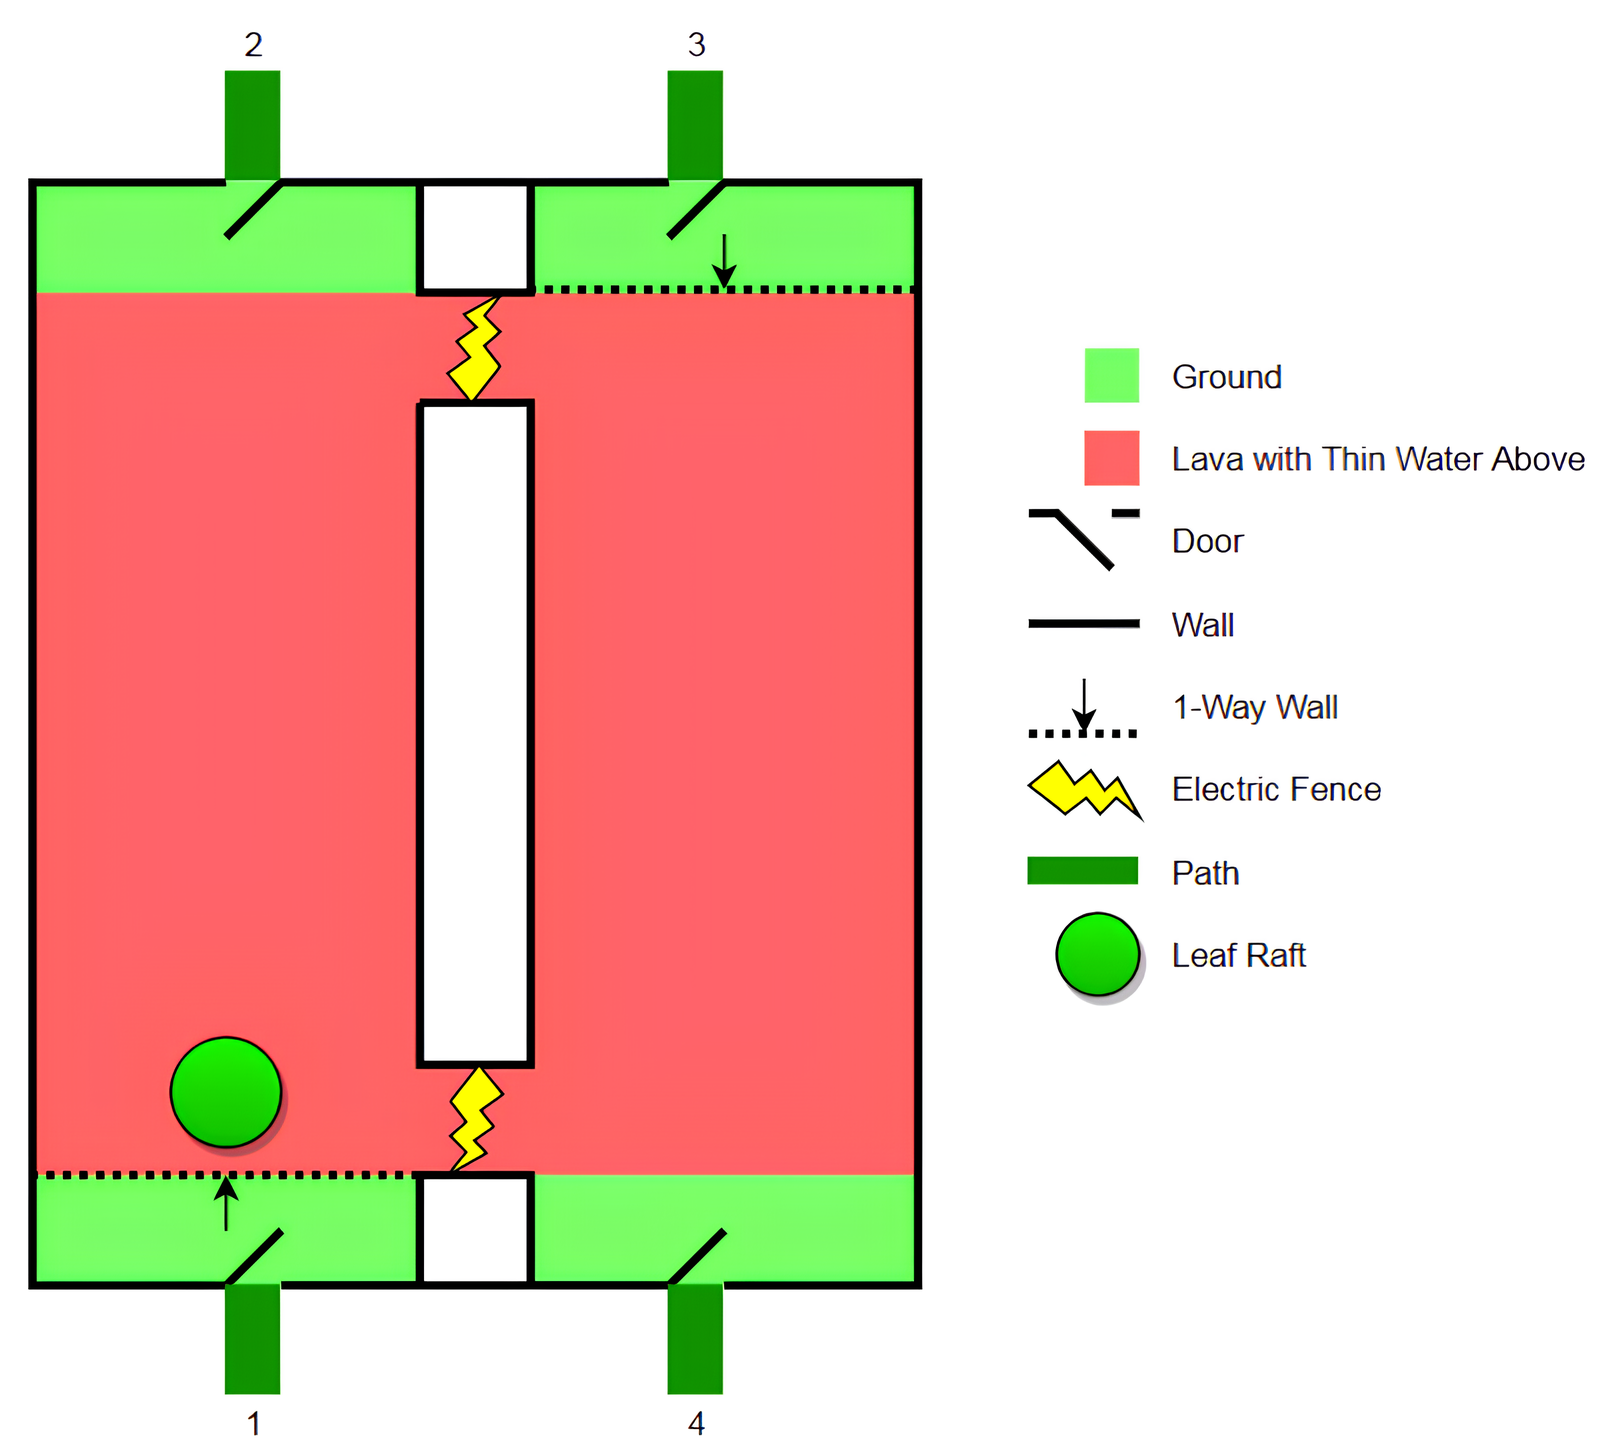
\includegraphics[width=0.8\textwidth]{res/Super Mario Galaxy 2.png}}
    \only<2>{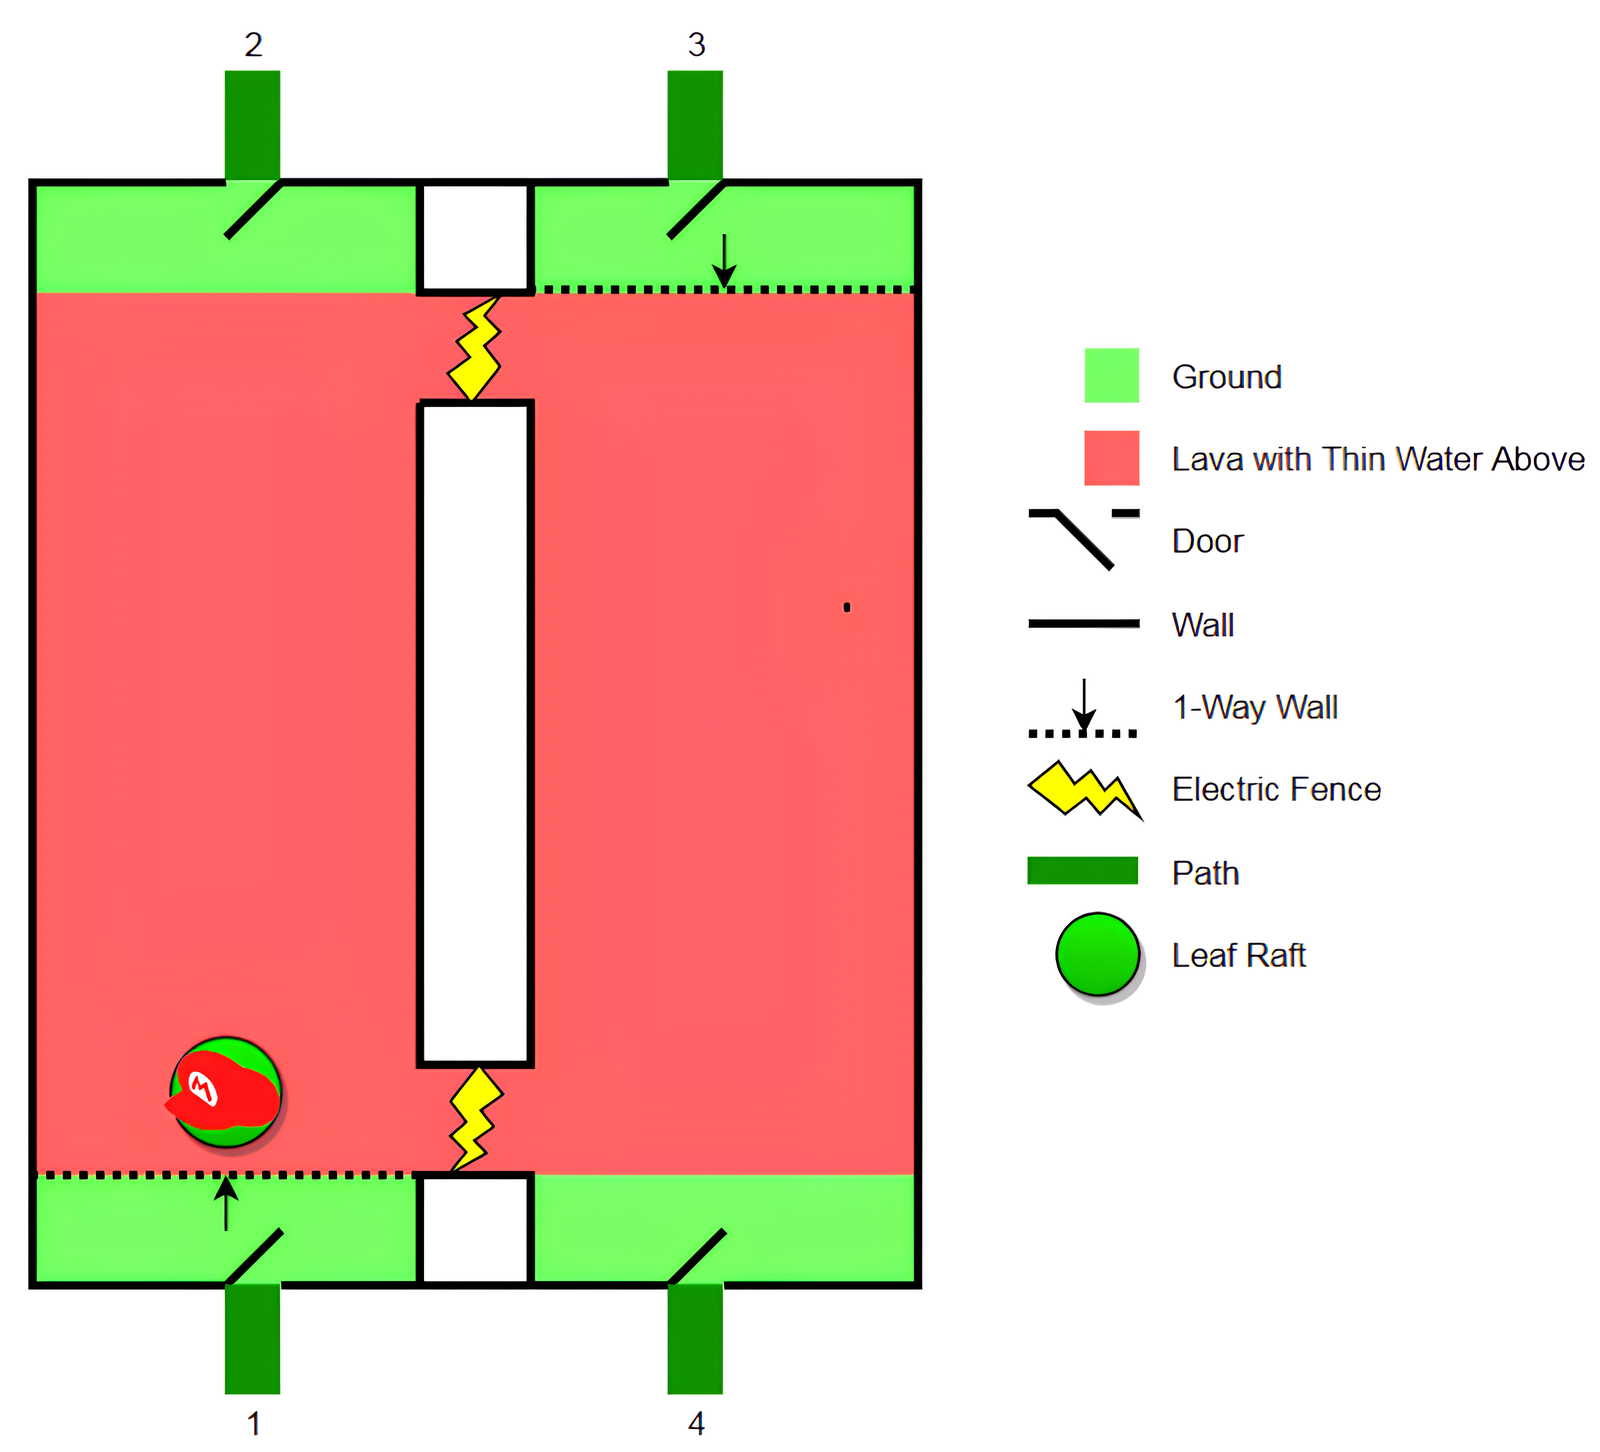
\includegraphics[width=0.8\textwidth]{res/Super Mario Galaxy 2 Anim1.png}}
    \only<3>{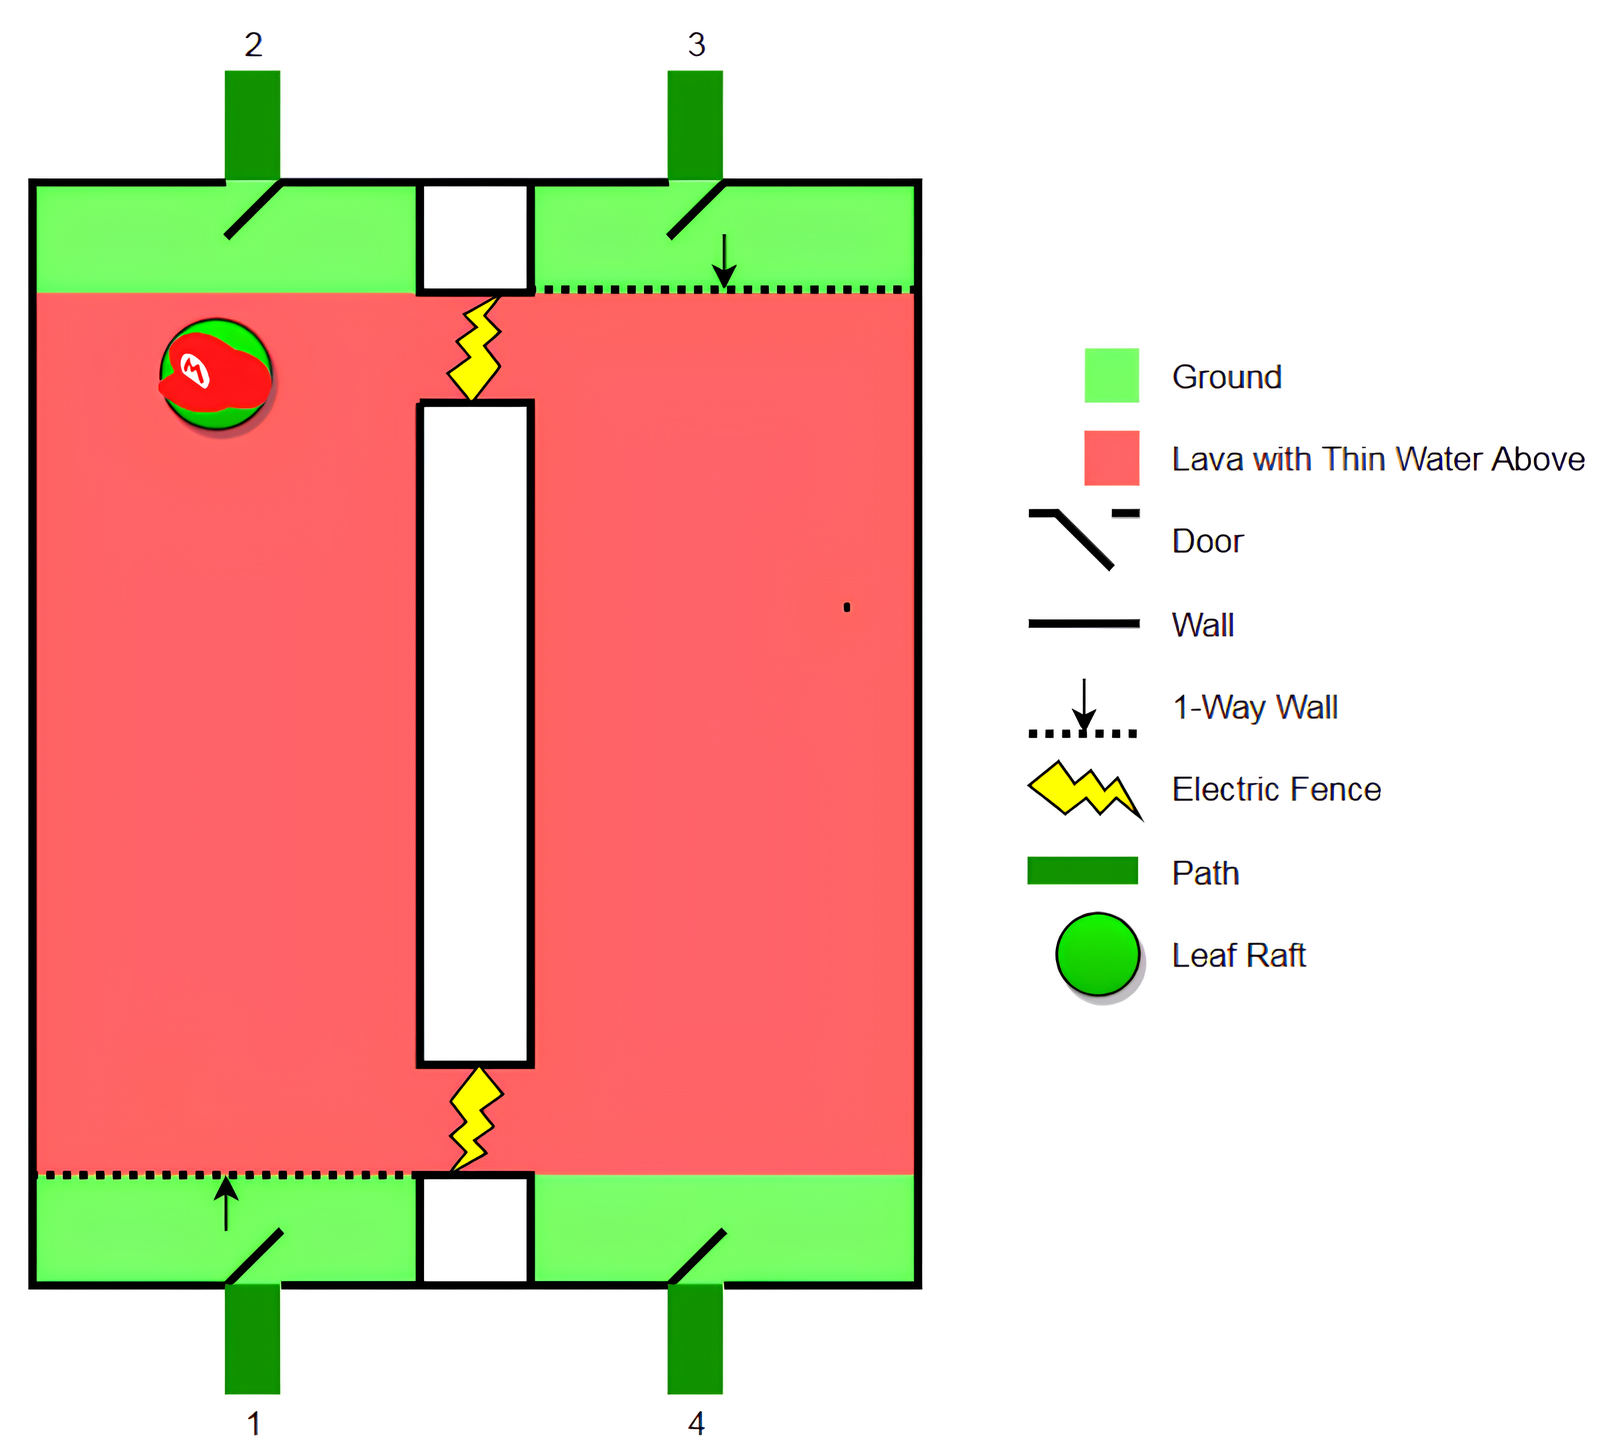
\includegraphics[width=0.8\textwidth]{res/Super Mario Galaxy 2 Anim2.png}}
    \only<4>{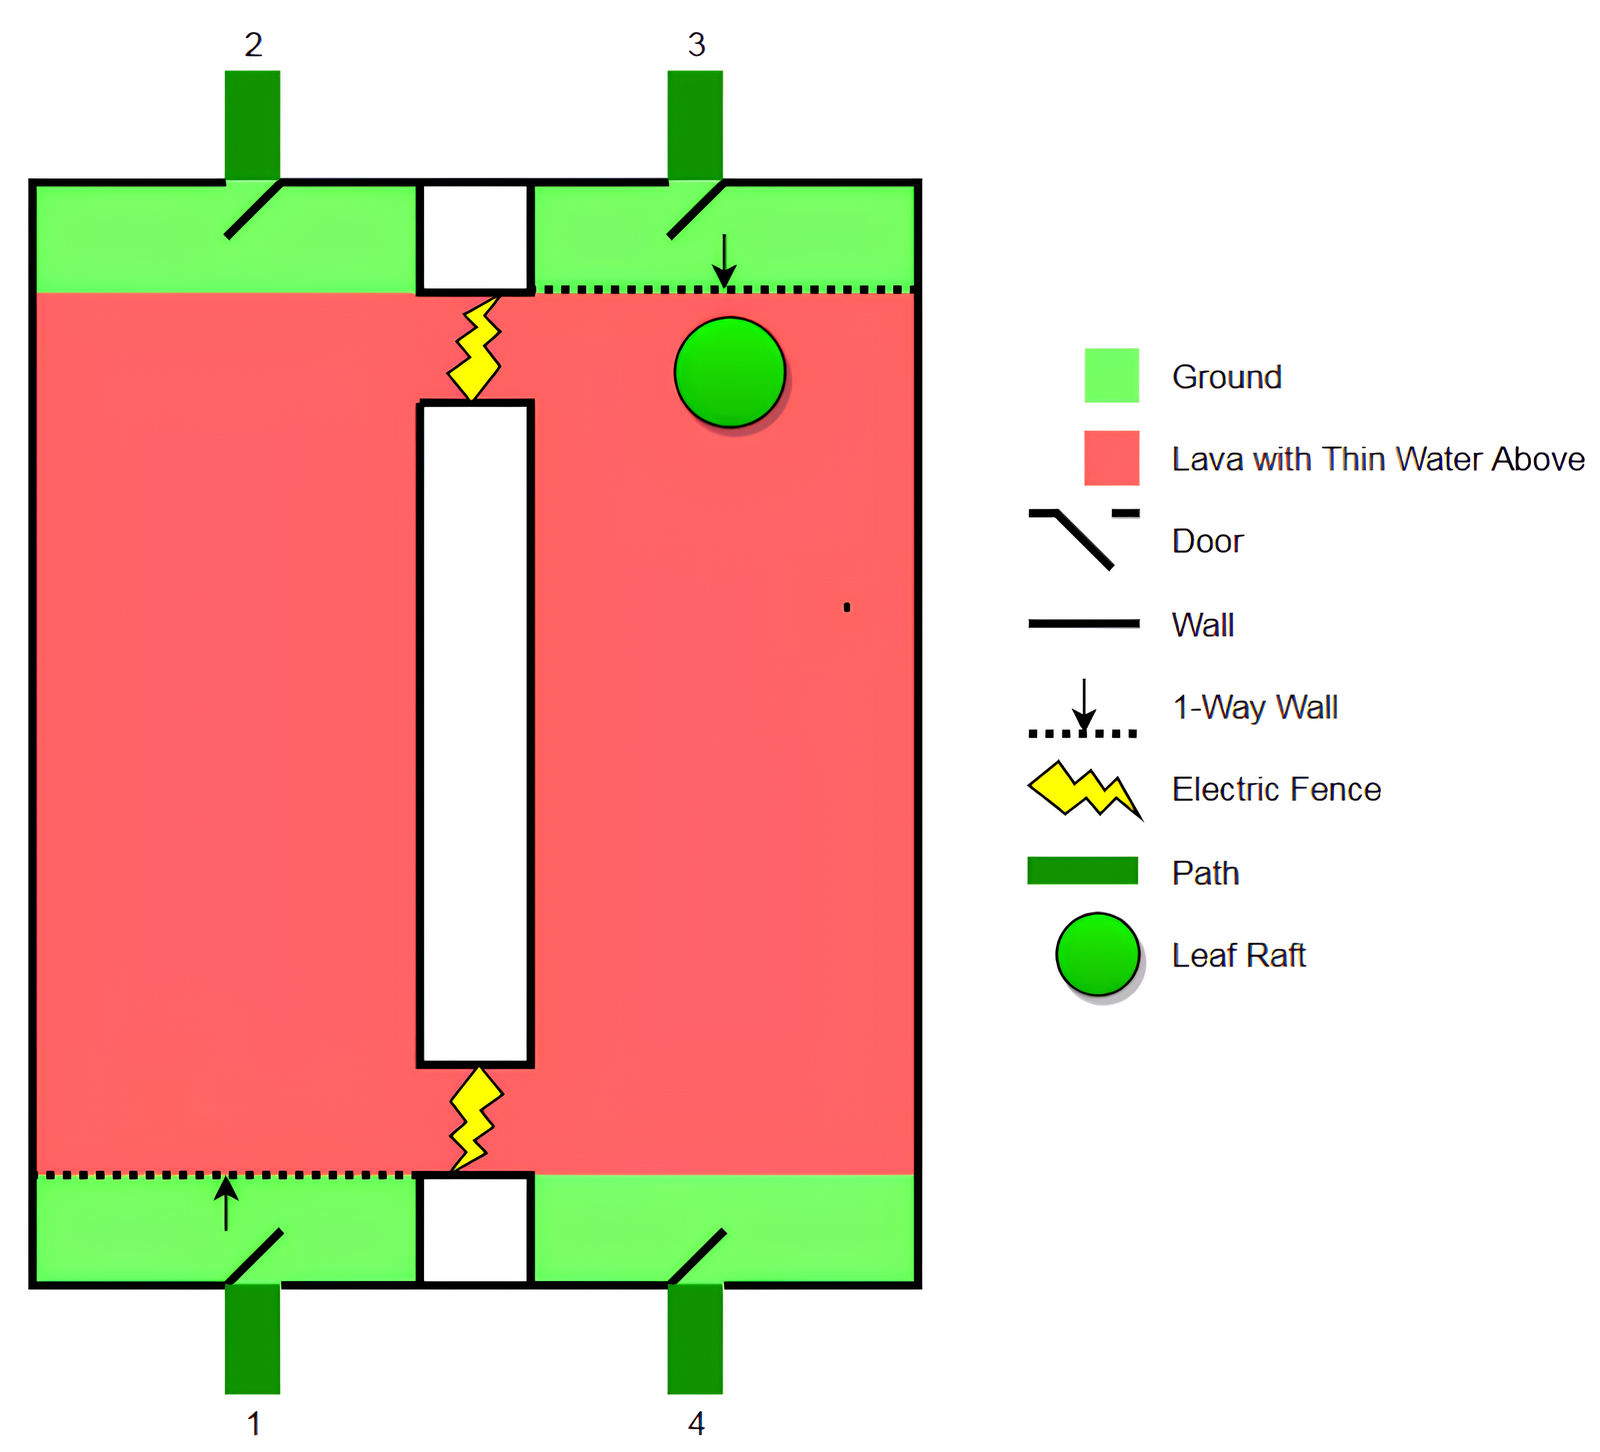
\includegraphics[width=0.8\textwidth]{res/Super Mario Galaxy 2 Anim3.png}}
  \end{center}
\end{frame}

\begin{frame}
  \frametitle{Similar constructs}
  \only<1>{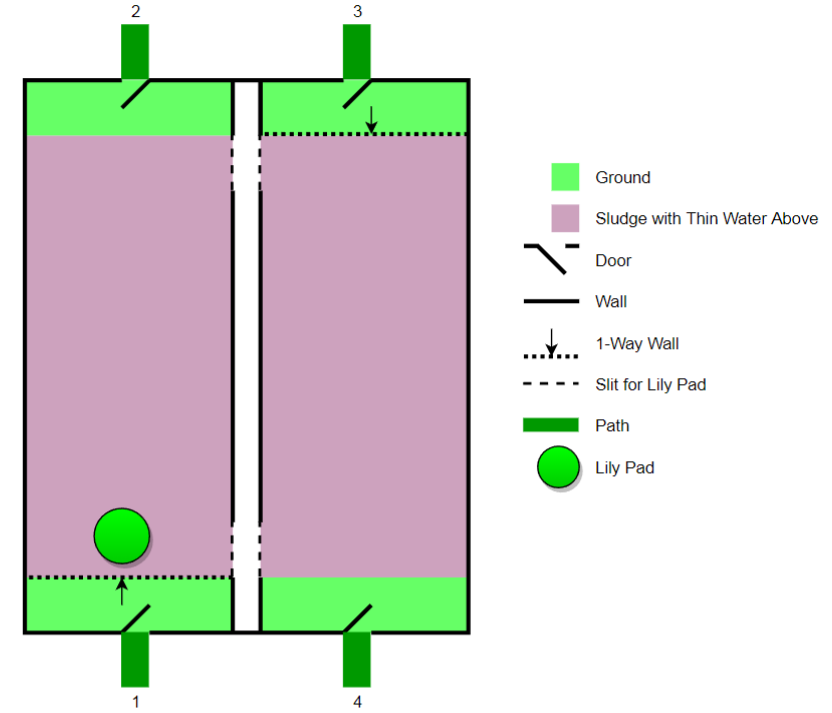
\includegraphics[width=0.8\textwidth]{res/Super Mario Sunshine.png}}
  \only<2>{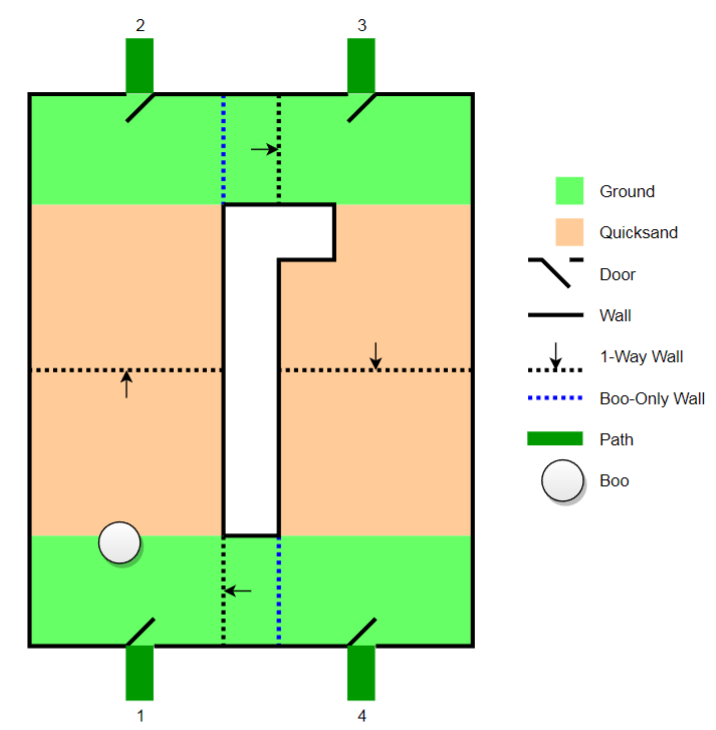
\includegraphics[width=0.8\textwidth]{res/Super Mario 64.png}}
\end{frame}

\subsection{Super Mario Galaxy is PSPACE-Hard}
\begin{frame}
  \frametitle{Super Mario Galaxy is PSpace-hard}
  \only<1>{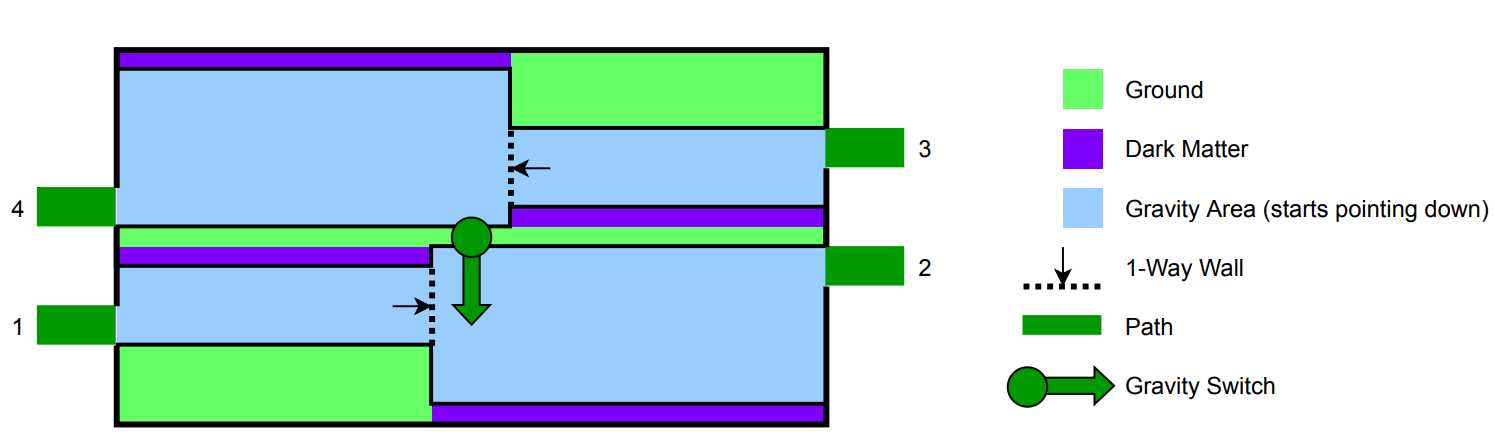
\includegraphics[width=1.1\textwidth]{res/Super Mario Galaxy.png}}
  \only<2>{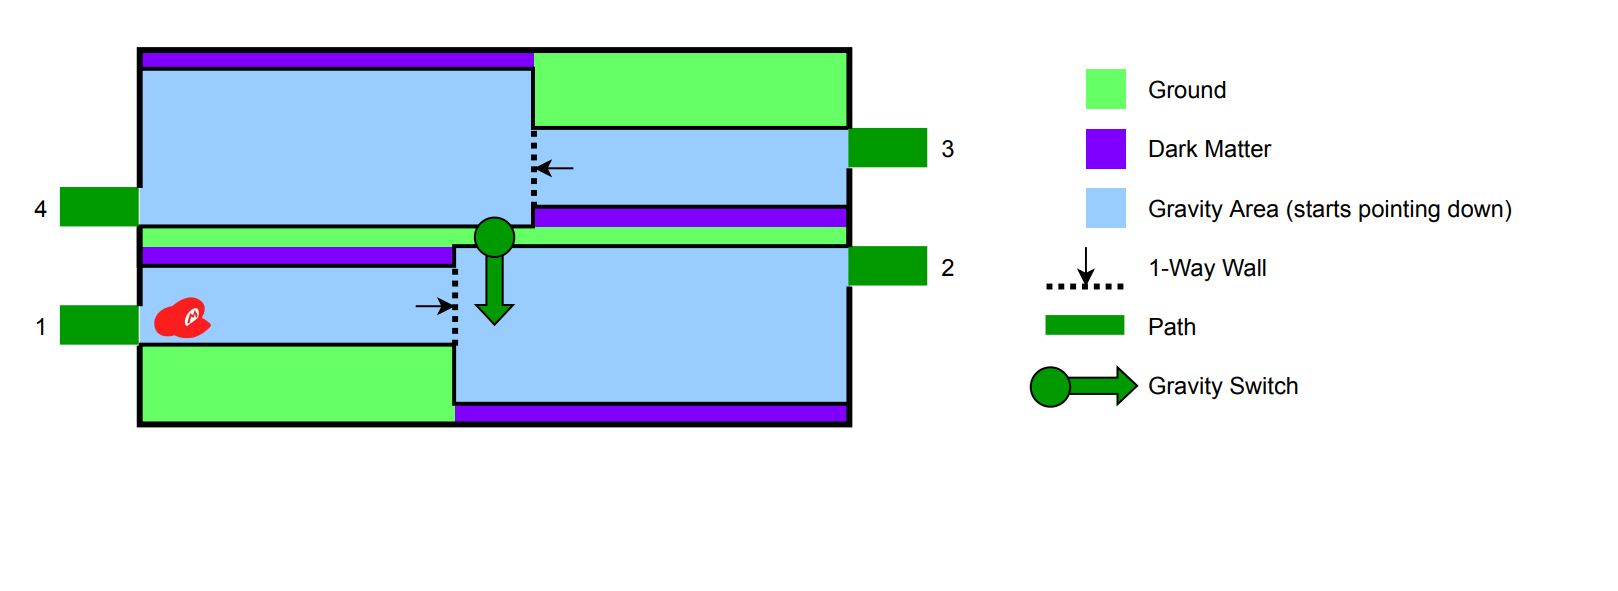
\includegraphics[width=1.1\textwidth]{res/Super Mario Galaxy Anim1.png}}
  \only<3>{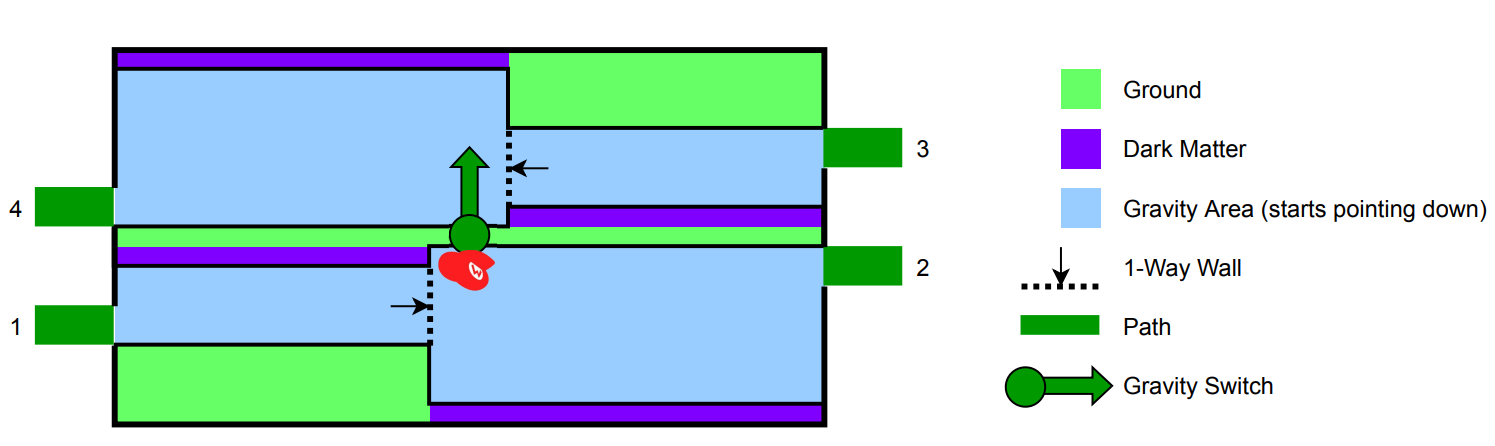
\includegraphics[width=1.1\textwidth]{res/Super Mario Galaxy Anim2.png}}
  \only<4>{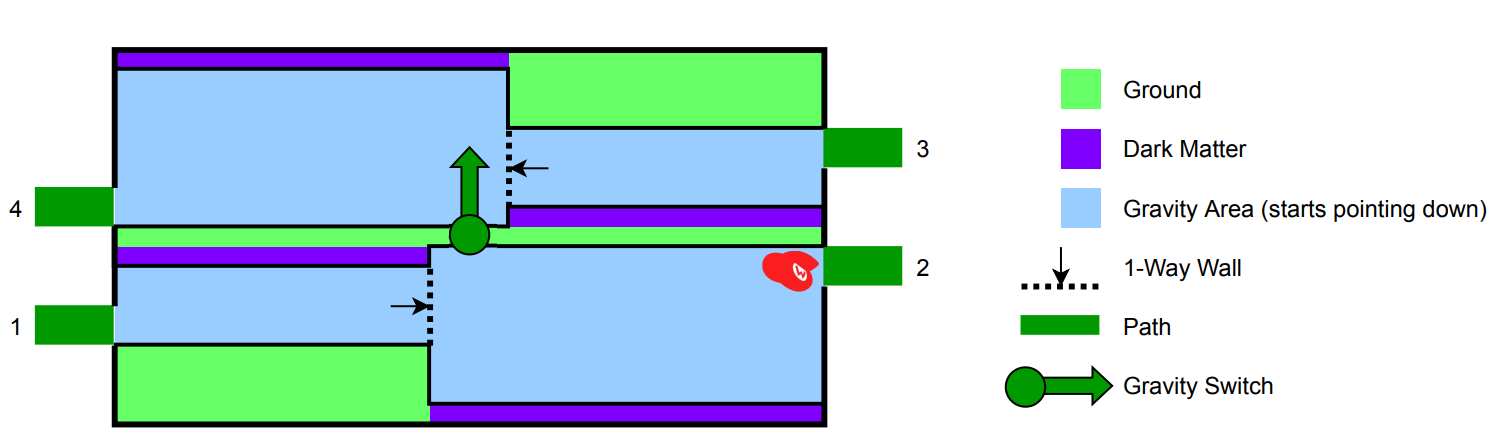
\includegraphics[width=1.1\textwidth]{res/Super Mario Galaxy Anim3.png}}
\end{frame}

\subsection{Super Mario Odessy is PSPACE-Hard}
\begin{frame}
  \frametitle{Super Mario Odessy is PSpace-hard}
  \only<1>{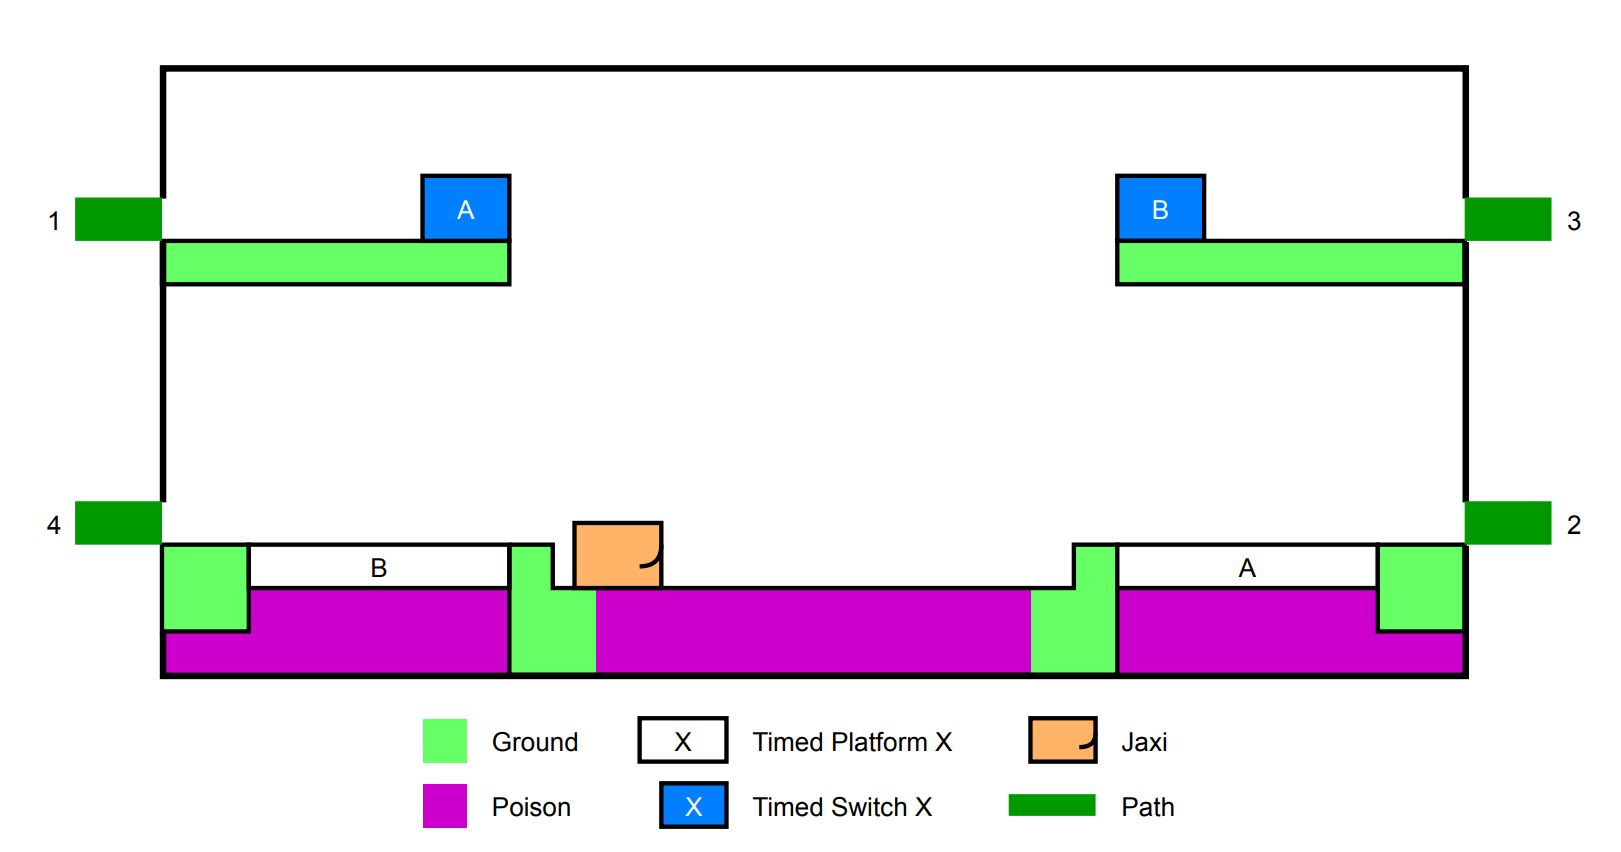
\includegraphics[width=1.05\textwidth]{res/Super Mario Odyssey.png}}
  \only<2>{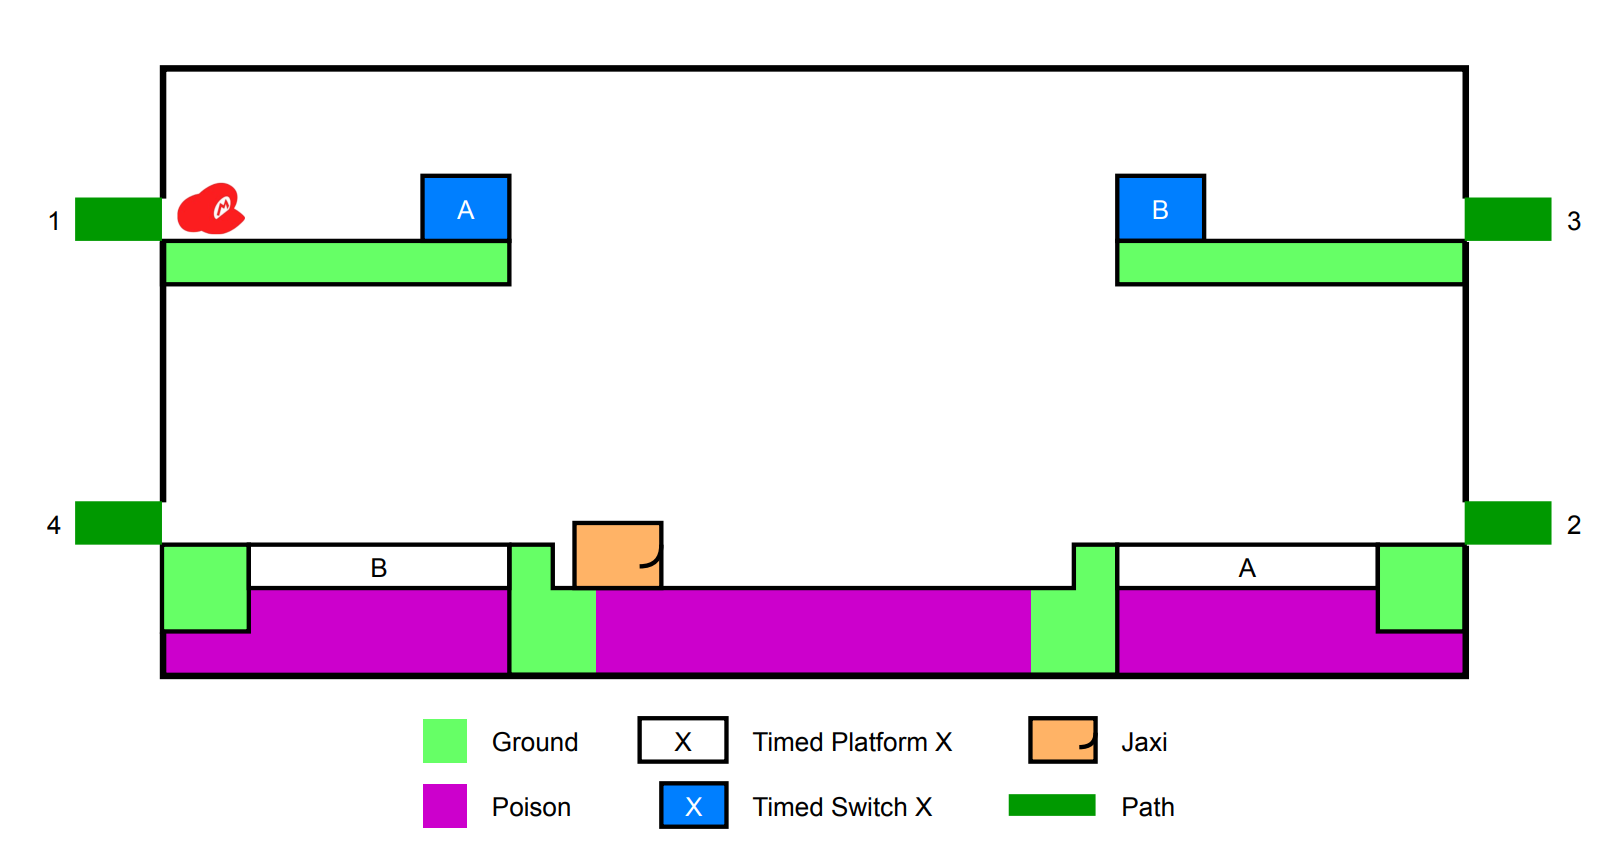
\includegraphics[width=1.05\textwidth]{res/Super Mario Odyssey Anim1.png}}
  \only<3>{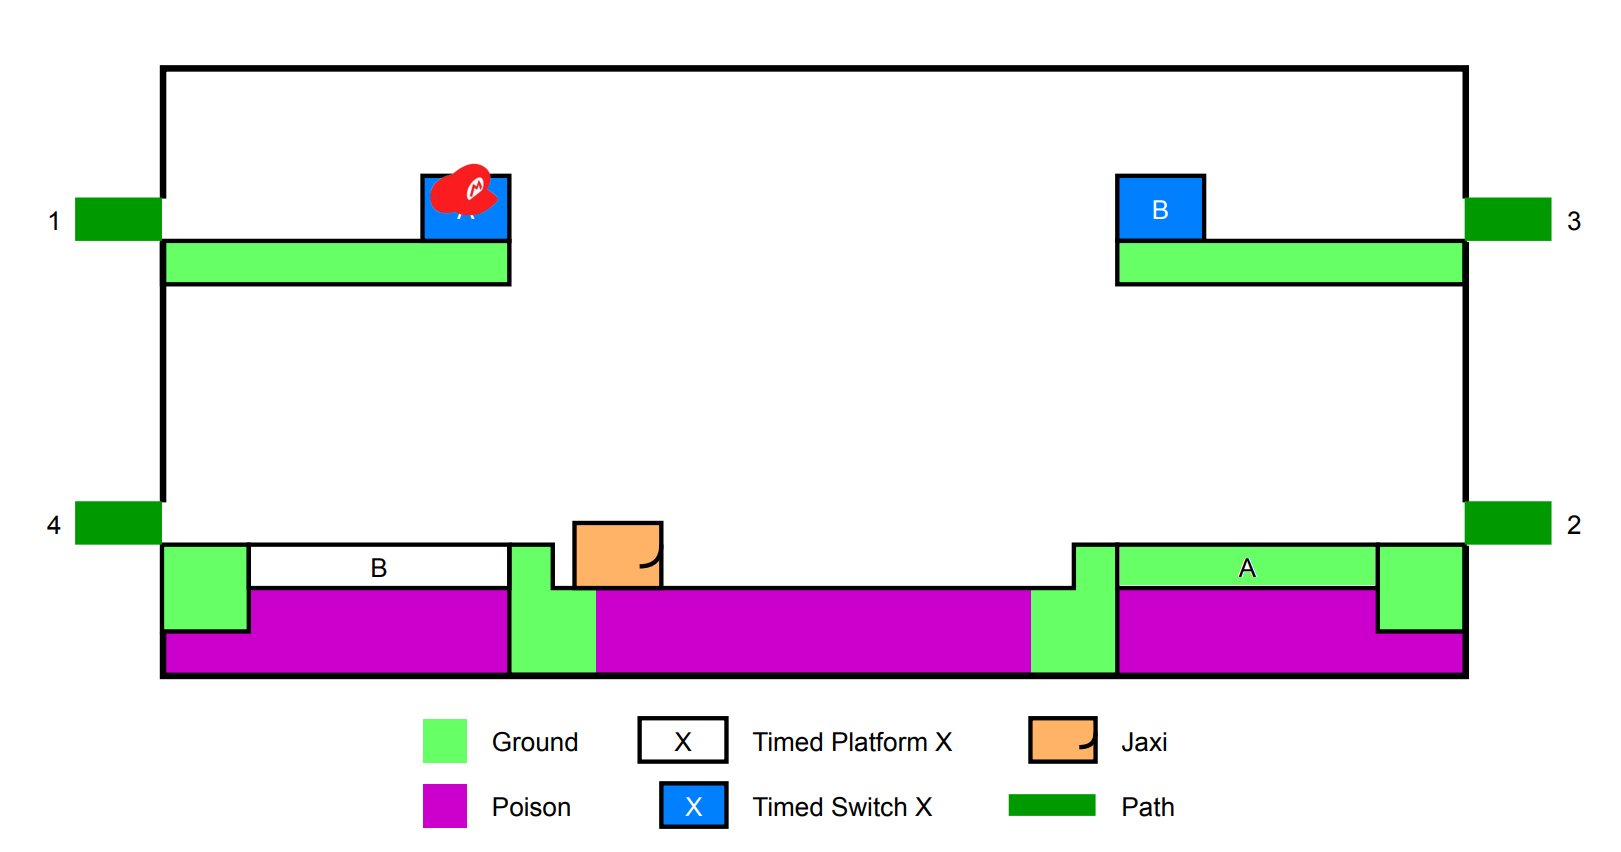
\includegraphics[width=1.05\textwidth]{res/Super Mario Odyssey Anim2.png}}
  \only<4>{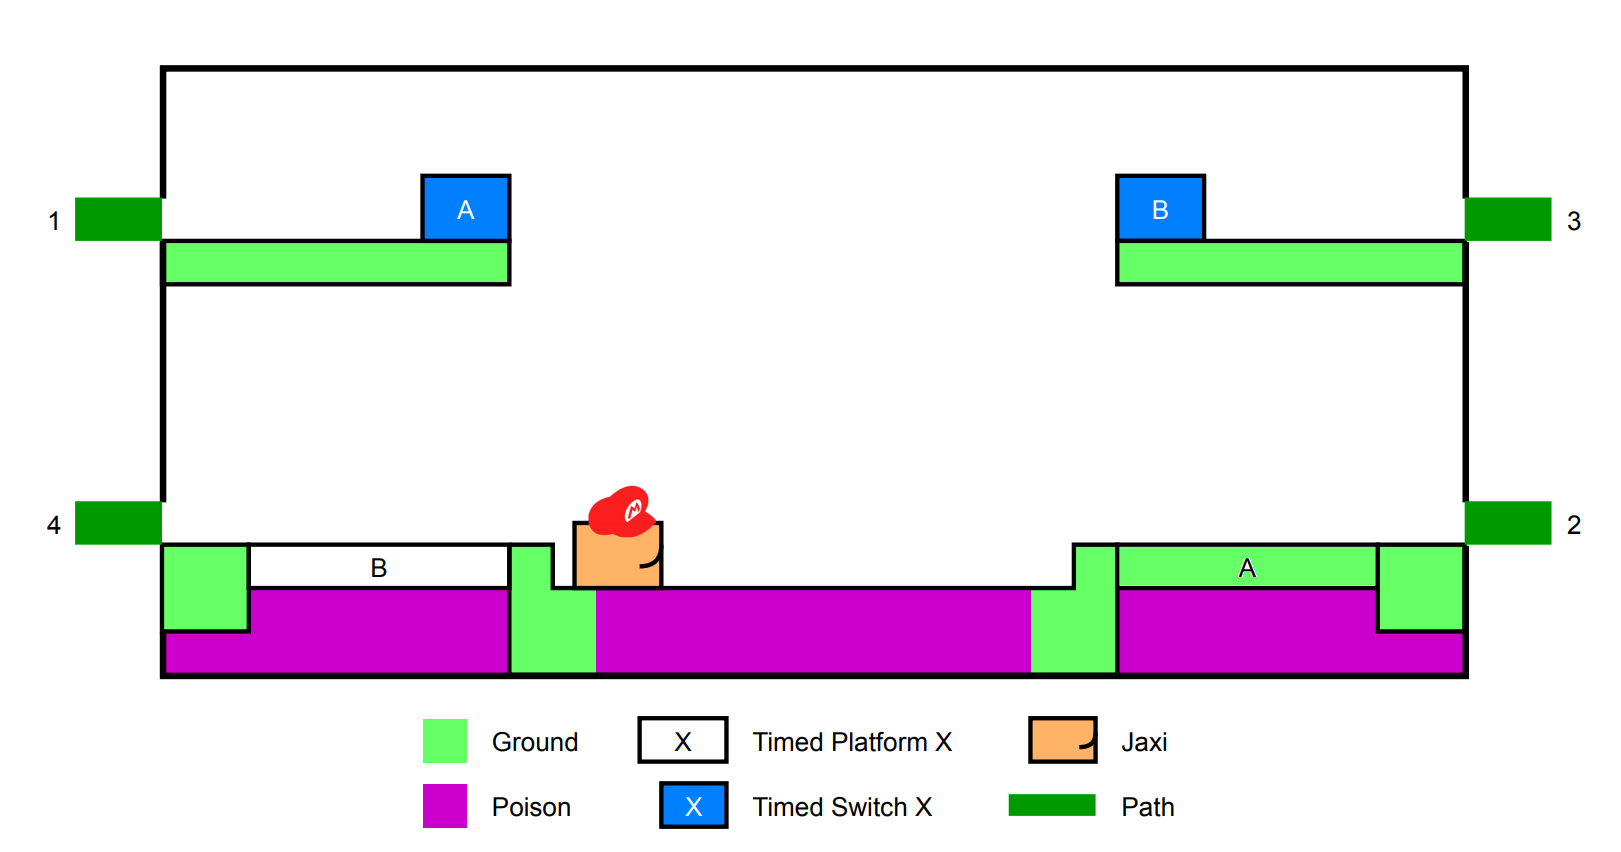
\includegraphics[width=1.05\textwidth]{res/Super Mario Odyssey Anim3.png}}
  \only<5>{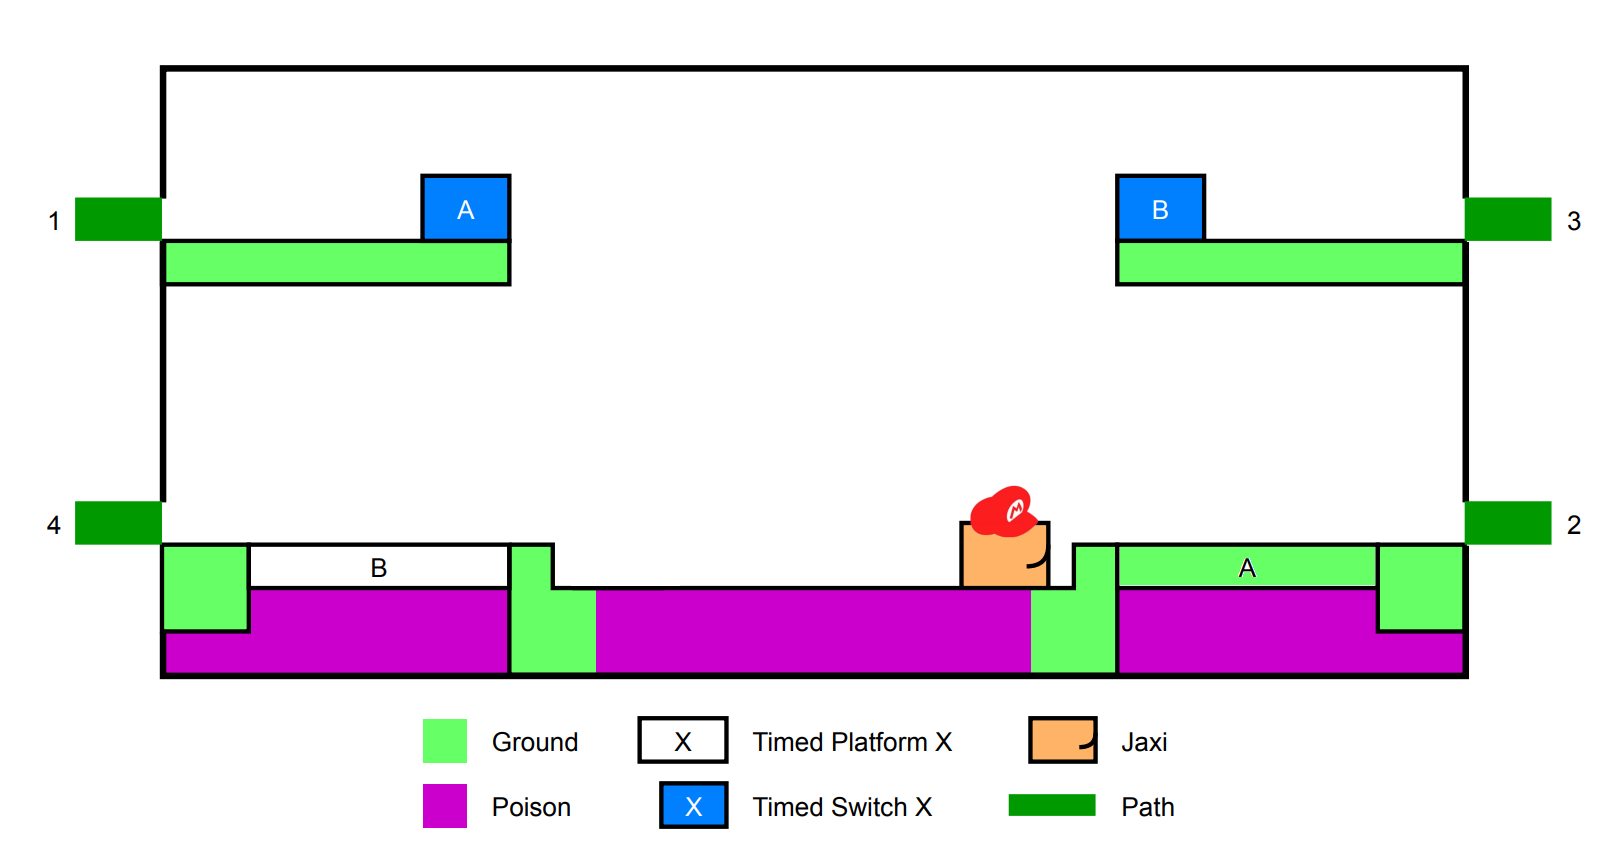
\includegraphics[width=1.05\textwidth]{res/Super Mario Odyssey Anim4.png}}
  \only<6>{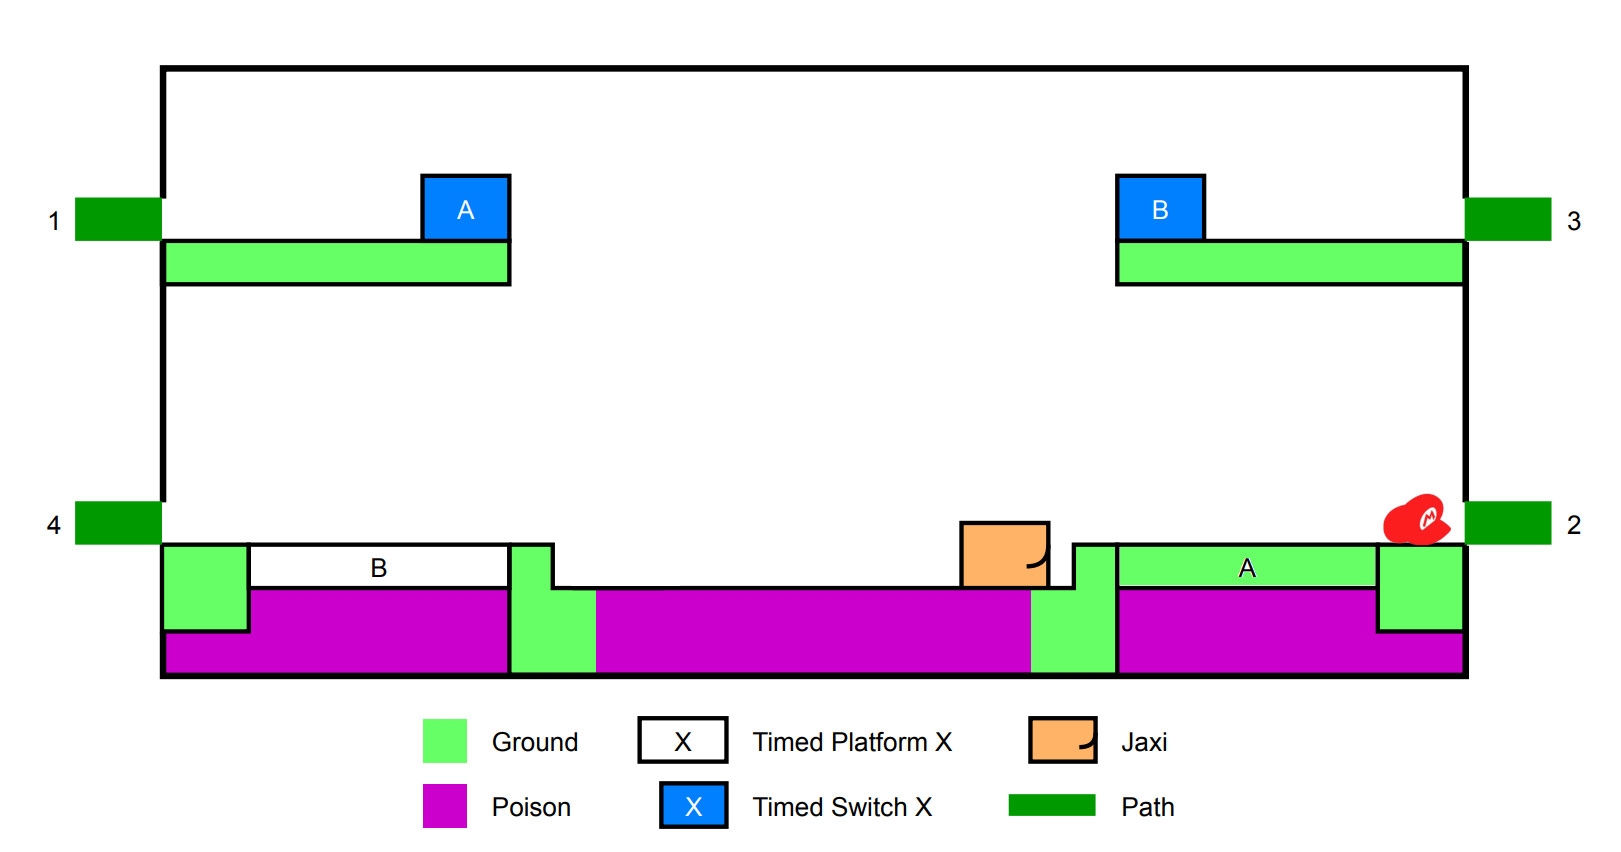
\includegraphics[width=1.05\textwidth]{res/Super Mario Odyssey Anim5.png}}
  \only<7>{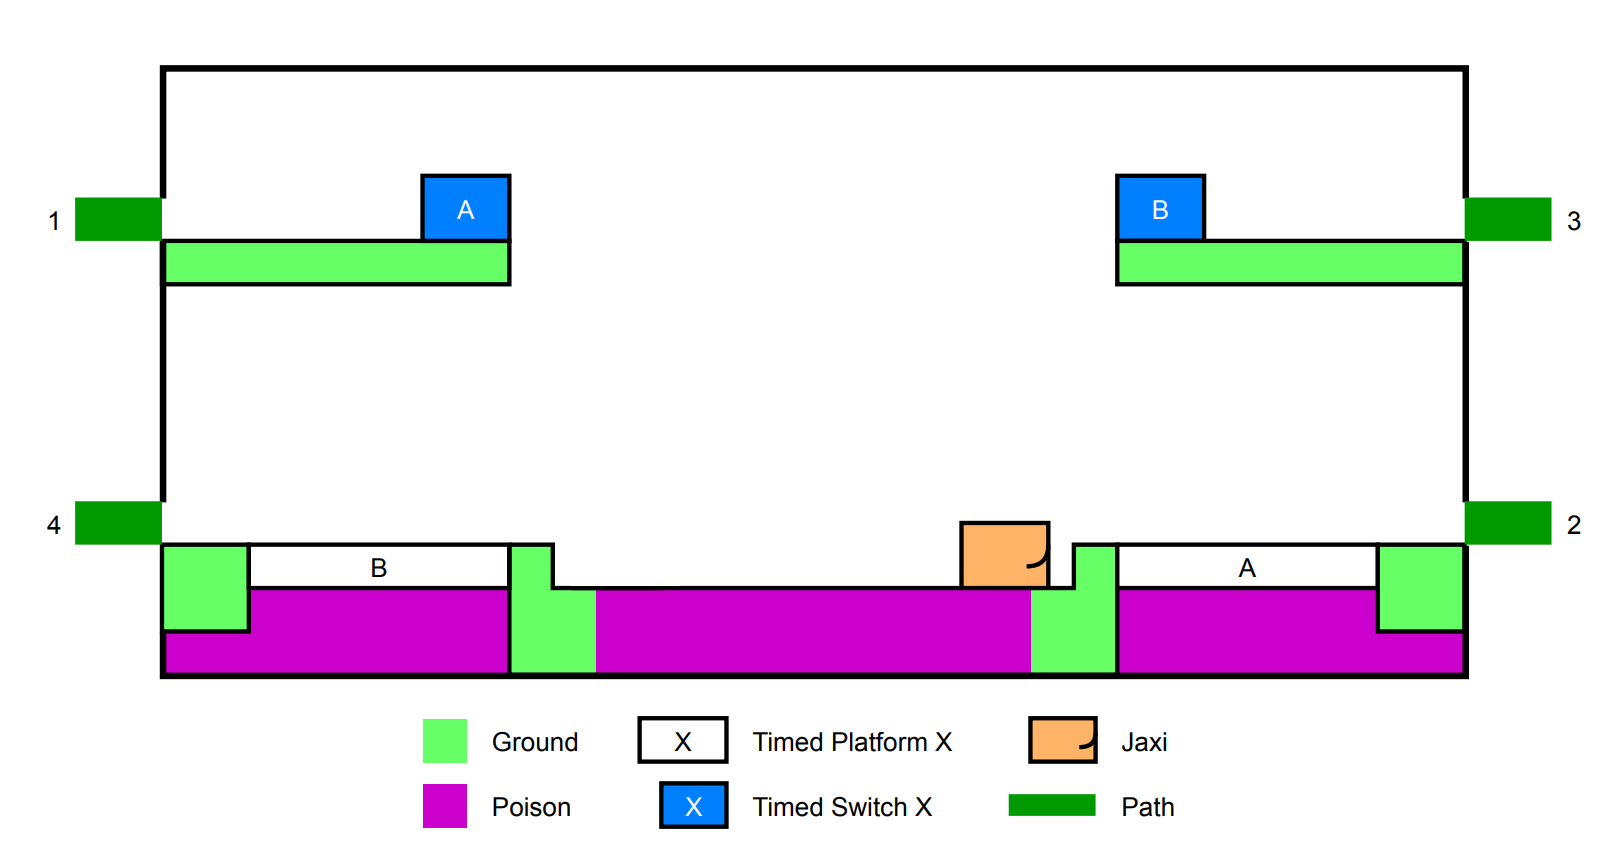
\includegraphics[width=1.05\textwidth]{res/Super Mario Odyssey Anim6.png}}
\end{frame}
\end{document}